
% Ok Fuck. I guess next quarter, try to start with unicode math. Also, you aren't allowed to change the matrix typeface anymore...


% Note for any github stalkers. I am currently in the process
% of learning LaTeX. I don't know what I'm doing yet. Sorry
% if my code absolutely sucks.
\documentclass{book}

\usepackage{fontspec} % used to import Calibri
\usepackage{anyfontsize} % used to adjust font size

% needed for inch and other length measurements
% to be recognized
\usepackage{calc}

% for colors and text effects as is hopefully obvious
\usepackage[dvipsnames]{xcolor}
\usepackage{soul}

% control over margins
\usepackage[margin=1in]{geometry}
\usepackage[strict]{changepage}

\usepackage{mathtools}
\usepackage{amsfonts}
\usepackage{bm}
\usepackage{amssymb} % originally imported to get the proof square
\usepackage[overcommands]{overarrows} % Get my preferred vector arrows...
\usepackage{relsize}
\usepackage{xfrac}

% Just am using this to get a dashed line in a table...
% Also you apparently want this to be inactive if you aren't
% using it because it slows compilation.
\usepackage{arydshln} \ADLinactivate 
\newenvironment{allowTableDashes}{\ADLactivate}{\ADLinactivate}

\usepackage{graphicx}
\graphicspath{{./158_Images/}}

\usepackage{tikz}
   \usetikzlibrary{arrows.meta}

\newfontfamily{\calibri}{Calibri}
\setlength{\parindent}{0pt}
\definecolor{RawerSienna}{HTML}{945D27}
\setul{0.14em}{0.07em}

\newcommand{\hOne}{%
   \color{Black}%
   \fontsize{14}{16}\selectfont%
}
\newcommand{\hTwo}{%
   \color{MidnightBlue}%
   \fontsize{13}{15}\selectfont%
}
\newcommand{\hThree}{%
   \color{PineGreen}
   \fontsize{13}{15}\selectfont%
}
\newcommand{\hFour}{%
   \color{Cerulean}
   \fontsize{12}{14}\selectfont%
}
\newcommand{\myComment}{%
   \color{RawerSienna}%
   \fontsize{12}{14}\selectfont%
}
\newcommand{\teachComment}{
   \color{Orange}%
   \fontsize{12}{14}\selectfont%
}
\newcommand{\exOne}{%
   \color{Purple}%
   \fontsize{14}{16}\selectfont%
}
\newcommand{\exTwo}{%
   \color{RedViolet}%
   \fontsize{13}{15}\selectfont%
}
\newcommand{\exP}{%
   \color{VioletRed}%
   \fontsize{12}{14}\selectfont%
}

\newenvironment{myIndent}{%
   \begin{adjustwidth}{2.5em}{0em}%
}{%
   \end{adjustwidth}%
}
\newenvironment{myDindent}{%
   \begin{adjustwidth}{5.0em}{0em}%
}{%
   \end{adjustwidth}%
}
\newenvironment{myTindent}{%
   \begin{adjustwidth}{7.5em}{0em}%
}{%
   \end{adjustwidth}%
}

\newenvironment{myConstrict}{%
   \begin{adjustwidth}{2.5em}{2.5em}%
}{%
   \end{adjustwidth}%
}

\newcommand{\udefine}[1]{%
   {\setulcolor{Red}%
   \setul{0.14em}{0.07em}%
   \ul{#1}}%
}

\newcommand{\uuline}[2][.]{%
{\vphantom{a}\color{#1}%
\rlap{\rule[-0.18em]{\widthof{#2}}{0.06em}}%
\rlap{\rule[-0.32em]{\widthof{#2}}{0.06em}}}%
#2}

\newcounter{LectureNumber}
\newcommand*{\markLecture}[1]{%
   \stepcounter{LectureNumber}%
   {\huge \color{Black} \textbf{Lecture \theLectureNumber: #1} \newline}%
}

\newcommand{\cyPen}[1]{{\vphantom{.}\color{Cerulean}#1}}

\newcommand{\pprime}{{\prime\prime}}
\newcommand{\suchthat}{ \hspace{0.5em}s.t.\hspace{0.5em}}
\newcommand{\rea}[1]{\mathrm{Re}(#1)}
\newcommand{\ima}[1]{\mathrm{Im}(#1)}
\newcommand{\comp}{\mathsf{C}}

\newcommand{\Proj}[2]{\mathrm{Proj}_{#2}(#1)}
\newcommand{\rank}[1]{\mathrm{rank}(#1)}
\newcommand{\nullity}[1]{\mathrm{nullity}(#1)}
\newcommand{\spanLA}[1]{\mathrm{span}\{#1\}}


\newcounter{PropNumber}
\newcommand{\propCount}{%
   \stepcounter{PropNumber}%
   \thePropNumber%
}

\newcommand{\mySepOne}[1][.]{%
   {\noindent\color{#1}{\rule{6.5in}{1mm}}}\\%
}
\newcommand{\mySepTwo}[1][.]{%
   {\noindent\color{#1}{\rule{6.5in}{0.5mm}}}\\%
}

\newenvironment{myClosureOneOld}[2][.]{%
   \color{#1}%
   \begin{tabular}{|p{#2in}|} \hline \\%
}{%
   \\ \\ \hline \end{tabular}%
}

\newenvironment{myClosureOne}[2][.]{%
   \color{#1}%
   \begin{tabular}{|p{#2in}|} \hline \\%
}{%
   \\ \hline \end{tabular}%
}

\newcommand{\retTwo}{\hfill\bigbreak}
\newcommand{\myVS}{\vphantom{$\int_a^b$}}
\newcommand{\myMathVS}{\vphantom{\int_a^b}}


% Hopefully this will be good enough
\NewOverArrowCommand{myVector}{%
   start = {{\smallermathstyle\relbar}},
   middle = {{\smallermathstyle\relbar}},
   end={{\rightharpoonup}}, space before arrow=0.15em,
   space after arrow=-0.045em,
}

\NewOverArrowCommand{myBar}{%
   start = {{\relbar}},
   middle = {{\relbar}},
   end={{\relbar}}, space before arrow=0em,
   space after arrow=-0.13em,
}

\newcommand{\mVec}[1]{\myVector{#1}}
\newcommand{\mVecAst}[1]{\myVector*{#1}}
\newcommand{\mMat}[1]{\mathbf{#1}}

% Programming stuff:
% ~~~~~~~~~~~~~~~~~~~~~~~~~~~~~~~~~~~~~~~~~~~~~~~~~~~~~~~~~~~~~~~~~~~~~
\usepackage{listings} % for writing code...
\lstset{
   basicstyle=\ttfamily
}

\colorlet{currentIdentifierFromLst}{Black}

\lstdefinestyle{170test}{
   basicstyle=\normalsize\ttfamily\color{Black},
   language=MATLAB,
   backgroundcolor = \color{Dandelion!5},
   commentstyle=\color{OliveGreen},
   keywordstyle=\color{Cerulean},
   numbersep=5pt,
   numbers=left,
   numberstyle=\color{Gray},
   tabsize=3,
   identifierstyle=\color{RedViolet},
   stringstyle=\color{BrickRed},
   showstringspaces=false,
   %morestring=[b]"
}
\newcommand{\lstSetTest}{%
   \lstset{style=170test}%
   \colorlet{currentIdentifierFromLst}{RedViolet}%
}

\newcommand{\identifier}[1]{%
   {\color{currentIdentifierFromLst}\texttt{#1}}%
}
% ~~~~~~~~~~~~~~~~~~~~~~~~~~~~~~~~~~~~~~~~~~~~~~~~~~~~~~~~~~~~~~~~~~~~~



\title{Math 170A Lecture Notes (Professor: Lei Huang)}
\author{Isabelle Mills}

\begin{document}
   \lstSetTest
   \maketitle
   \calibri

   {\huge \color{Black} \textbf{Week 1 Notes (1/8 - 1/12/2024)}%
   \stepcounter{LectureNumber}%
   \stepcounter{LectureNumber}%
   \stepcounter{LectureNumber} \retTwo}
   
   \hOne
   For this class, we shall define the number of \udefine{flops} an
   algorithm takes as the number of individual $+$, $-$, $\times$, $/$,
   and $\sqrt{\phantom{x}}$ operations on \uuline{real numbers}
   used in the algorithm. \retTwo
   
   \begin{myIndent} \hTwo
      For example: taking the inner product of two vectors
      $\mVec{u} = (u_1, u_2, \ldots, u_n)$ and
      $\mVec{v} = (v_1, v_2, \ldots, v_n)$ requires
      $n$ multiplications and $(n-1)$ additions. So we'll say
      it has a flops count of $2n-1$.
   \end{myIndent}
   \hOne
   \retTwo

   Technically, the word "flop" stands for 
   \textul{floating (point) operation}. Based on that knowledge,
   hopefully it is easier to guess what is and is not a flop. For
   instance, observe the code written below for taking an inner
   product of two $n$-vectors.

   \begin{tabular}{ p{3.0in} p{3.0in}}
      \retTwo
      \begin{lstlisting}
   P = 0
   for i = 1:n
      P = P + v(i) * w(i)
   end
      \end{lstlisting}
      &
      \begin{myIndent} 
         {\hTwo Neither incrementing \identifier{i} nor \newline
         initializing any other variables are counted towards the 
         flop number. Because the code does \identifier{n} additions
         and multiplications between \newline floating point
         numbers, we say this function has $2n$ flops.}
      \end{myIndent}
   \end{tabular}


   \mySepOne

   Here is how we formally define \udefine{Big-$\mathcal{O}$ Notation}:
   \retTwo
   For a sequence $a_n$, we define $a_n = \mathcal{O}(b_n)$ if there exists
   real constants\\ $C, N \geq 0$ such that for $n \geq N$, \hspace{0.25em}
   $a_n \leq Cb_n$.
   \retTwo

   \exOne
   \uuline{Example problem}:

   \begin{tabular}{ p{3.7in} p{2.4in} }
      \begin{lstlisting}
      function x = lowertriangsolve(L, b)
         N = size(L);
         n=size(b,1);
         x=b;
   
         for i=1:N(1):
            for j=1:i-1
               x(i) = x(i) - L(i,j)*x(j);
            end
   
            if L(i, j) == 0
               error('matrix is singular')
            end
            x(i) = x(i)/L(i,i);
         end
      end
      \end{lstlisting}
      &
      \exP
      Inside the main for loop (lines 6-15):
      \begin{myIndent}
         Line 8 has $2(\texttt{i}-1)$ flops.\newline
         Line 14 has an additional flop.\newline
      \end{myIndent}

      Thus, the total number of flops is:
      \[\sum_{\texttt{i}=1}^{n}(2\texttt{i}-1)
      = 2\left(\sum_{\texttt{i}=1}^{n}\texttt{i}\right) - n\]

      This then simplifies to:
      \[ 2\left( \dfrac{n(n+1)}{2} \right) - n
      = 1n^2 \]

      So \identifier{x} has $\mathcal{O}(n^2)$ flops as \identifier{n} goes
      to \newline infinity.
   \end{tabular}

   \newpage \hOne
   
   \markLecture{1/17/2024}

   Row operations used in Gaussian elemination can be represented via matrix \\multiplication as demonstrated below.
   
   {\hTwo
   \begin{allowTableDashes}
      \begin{tabular}{ p{4.4in};{10pt/3pt}p{1.6in} }
         {\center \phantom{ Matrix representation}\newline Action \par} & {\center Matrix representation \newline of the operation \newline \par} \\
         \hline {\hFour
         \[
         \begin{bmatrix}
            a_{1,1} & a_{1,2} & a_{1,3} & a_{1,4} \\
            a_{2,1} & a_{2,2} & a_{2,3} & a_{2,4} \\
            a_{3,1} & a_{3,2} & a_{3,3} & a_{3,4} \\
            a_{4,1} & a_{4,2} & a_{4,3} & a_{4,4}
         \end{bmatrix} \xlongrightarrow{R_2 \leftrightarrow R_3}
         \begin{bmatrix}
            a_{1,1} & a_{1,2} & a_{1,3} & a_{1,4} \\
            a_{3,1} & a_{3,2} & a_{3,3} & a_{3,4} \\
            a_{2,1} & a_{2,2} & a_{2,3} & a_{2,4} \\
            a_{4,1} & a_{4,2} & a_{4,3} & a_{4,4}
         \end{bmatrix} \]} & {\hFour
         \[
         \begin{bmatrix}
            1 & 0 & 0 & 0 \\
            0 & 0 & 1 & 0 \\
            0 & 1 & 0 & 0 \\
            0 & 0 & 0 & 1
         \end{bmatrix}\]}
         \\
         \hline {\hFour
         \[
         \begin{bmatrix}
            a_{1,1} & a_{1,2} & a_{1,3} & a_{1,4} \\
            a_{2,1} & a_{2,2} & a_{2,3} & a_{2,4} \\
            a_{3,1} & a_{3,2} & a_{3,3} & a_{3,4} \\
            a_{4,1} & a_{4,2} & a_{4,3} & a_{4,4}
         \end{bmatrix} \xlongrightarrow{\frac{2}{3}R_2 \rightarrow R_2}
         \begin{bmatrix}
            a_{1,1} & a_{1,2} & a_{1,3} & a_{1,4} \\
            \frac{2}{3}a_{2,1} & \frac{2}{3}a_{2,2} & \frac{2}{3}a_{2,3} & \frac{2}{3}a_{2,4} \\
            a_{3,1} & a_{3,2} & a_{3,3} & a_{3,4} \\
            a_{4,1} & a_{4,2} & a_{4,3} & a_{4,4}
         \end{bmatrix} \]} & {\hFour
         \[
         \begin{bmatrix}
            1 & 0 & 0 & 0 \\
            0 & \frac{2}{3} & 0 & 0 \\
            0 & 0 & 1 & 0 \\
            0 & 0 & 0 & 1
         \end{bmatrix}\]}
         \\
         \hline {\hFour
         \[
         \begin{matrix}
            \begin{bmatrix}
               a_{1,1} & a_{1,2} & a_{1,3} & a_{1,4} \\
               a_{2,1} & a_{2,2} & a_{2,3} & a_{2,4} \\
               a_{3,1} & a_{3,2} & a_{3,3} & a_{3,4} \\
               a_{4,1} & a_{4,2} & a_{4,3} & a_{4,4}
            \end{bmatrix} \\
            \phantom{
               \text{\footnotesize $R_3 + \frac{2}{3}R_2 \rightarrow R_3$ }}
            {\left\downarrow \vphantom{{\int_A^\frac{\frac{\frac{A}{1}}{1}}{1}}} \right.}  \text{\footnotesize $R_3 + \frac{2}{3}R_2 \rightarrow R_3$ } \\
            \begin{bmatrix}
               a_{1,1} & a_{1,2} & a_{1,3} & a_{1,4} \\
               a_{2,1} & a_{2,2} & a_{2,3} & a_{2,4} \\
               a_{3,1} {+ \frac{2}{3}a_{2,1}}  & a_{3,2} {+ \frac{2}{3}a_{2,2}} & a_{3,3} {+ \frac{2}{3}a_{2,3}} & a_{3,4} {+ \frac{2}{3}a_{2,4}} \\
               a_{4,1} & a_{4,2} & a_{4,3} & a_{4,4}
            \end{bmatrix}
         \end{matrix}
         \]} & { \hFour \retTwo \retTwo 
         \[
         \begin{bmatrix}
            1 & 0 & 0 & 0 \\
            0 & 1 & 0 & 0 \\
            0 & \frac{2}{3} & 1 & 0 \\
            0 & 0 & 0 & 1
         \end{bmatrix}\]} 
      \end{tabular}
   \end{allowTableDashes}
   } \retTwo \retTwo

   The importance of representing elementary row operations as matrices is that we can multiply these representations together to compose rows operations. Thus, these representations are central to many matrix decompositions.

   
   \begin{myIndent}
      {\exTwo
         For example, we can represent turning a matrix into row echelon form as follows:
         \[
         \begin{bmatrix}
            1 & 0 & 0 \\
            0 & 1 & 0 \\
            0 & -\frac{2}{9} & 1
         \end{bmatrix}\begin{bmatrix}
            1 & 0 & 0 \\
            0 & 1 & 0 \\
            -2 & 0 & 1
         \end{bmatrix}\begin{bmatrix}
            1 & 0 & 0 \\
            -3 & 1 & 0 \\
            0 & 0 & 1
         \end{bmatrix}\begin{bmatrix}
            2 & 4 & 5 \\
            6 & 3 & 4 \\
            4 & 6 & 2
         \end{bmatrix} = \begin{bmatrix}
            2 & 4 & 5 \\
            0 & -9 & -11 \\
            0 & 0 & \frac{-50}{9}
         \end{bmatrix}\]
      }
   \end{myIndent}
   \newpage

   Here are some more observations about row operation matrices:
   
   \begin{itemize}
      \item Row scaling operations are represented by diagonal matrices and thus are also both lower and upper triangular.
      
      \item For $i<j$, adding a multiple of the $i$th row to the $j$th row is represented by a lower triangular matrix.
      
      \item For $i>j$, adding a multiple of the $i$th row to the $j$th row is represented by an upper triangular matrix.
      
      \item Row swaps are not represented as triangular matrices. However, they are\\ \uuline{permutation} matrices.
   \end{itemize} \retTwo

   Now note that in the normal algorithm for Gaussian elimination, assuming we never need to swap rows, all row operations will be such that their matrix representation is lower triangular. 
   
   \begin{myIndent} \hTwo
      Thus, given an invertible square matrix $\mMat{A}$, we can represent doing \\Gaussian elimination on $\mMat{A}$ by the equation: $\mMat{L}_n\mMat{L}_{n-1}\dotsb\mMat{L}_{2}\mMat{L}_{1}\mMat{A} = \mMat{U}$ where $\mMat{L}_i$ is a lower triangular matrix and $\mMat{U}$ is an upper triangular matrix. Then, because the product of two lower triangular matrices is also lower triangular, we can multiply all the lower triangular matries together to get an equation of the form $\mMat{L}\mMat{A}=\mMat{U}$. Finally, we multiply both sides of the equation on the left by $\mMat{L}^{-1}$ to get that\\ $\mMat{A}=\mMat{L}^{-1}\mMat{U}$. And as the inverse of a lower triangular matrix is also lower triangular, we know that we have decomposed $\mMat{A}$ into the product of a lower triangular matrix and an upper triangular matrix. This algorithm is called \udefine{LU decomposition}. \retTwo
   \end{myIndent}

   As for why we would want to use LU decomposition, we can look at the number of flops different matrix operations require.
   \hTwo
   \begin{myIndent}
      Assume we are given an invertible $n\times n$ matrix $\mMat{A}$ and two vectors $\mVec{x}, \mVec{b} \in \mathbb{R}^n$. \retTwo
      Firstly note that row reduction takes approximately $\frac{2}{3}n^3$ flops while the back\\ substitution algorithm takes approximately $n^2$ flops. Thus, for larger values of $n$, solving the matrix equation $\mMat{A}\mVec{x} = \mVec{b}$ takes around $\frac{2}{3}n^3$ flops. \retTwo

      Now lets compare this to the number of flops the best algorithm we can make to do LU decomposition takes.
      
      {\begin{myIndent} \hThree
         Assuming we don't need to do any row swaps, than the only elementary row operations we need to do are adding scaled rows to other rows. This is where our first optimization comes into play. The inverse of a row addition is merely a row subtraction. For example:
            {\begin{myTindent} \hThree
               $\begin{bmatrix}
                  1 & 0 & 0 \\
                  a & 1 & 0 \\
                  0 & 0 & 1
               \end{bmatrix}^{-1} = \begin{bmatrix}
                  1 & 0 & 0 \\
                  -a & 1 & 0 \\
                  0 & 0 & 1
               \end{bmatrix}$ \retTwo
            \end{myTindent}}

         \newpage
         Thus, we can fairly straightforwardly get an expression of the form \\$ \mMat{A} = \mMat{L}_1 \mMat{L}_2 \cdots \mMat{L}_k \mMat{U}$ by multiplying the inverse of each elementary row \\operation matrix to both sides of the equation representing the actions we took to reduce $\mMat{A}$ to $\mMat{U}$. \retTwo

         Now, we apply another two shortcuts to speed up our calculations. \retTwo Firstly, observe that:
         $
         \left[\begin{smallmatrix}
            1 & 0 & 0 & 0 \\
            0 & 1 & 0 & 0 \\
            0 & a & 1 & 0 \\
            0 & 0 & 0 & 1
         \end{smallmatrix}\right]
         \left[\begin{smallmatrix}
            1 & 0 & 0 & 0 \\
            0 & 1 & 0 & 0 \\
            0 & 0 & 1 & 0 \\
            0 & b & 0 & 1
         \end{smallmatrix}\right] = \left[\begin{smallmatrix}
            1 & 0 & 0 & 0 \\
            0 & 1 & 0 & 0 \\
            0 & 0 & 1 & 0 \\
            0 & b & 0 & 1
         \end{smallmatrix}\right]
         \left[\begin{smallmatrix}
            1 & 0 & 0 & 0 \\
            0 & 1 & 0 & 0 \\
            0 & a & 1 & 0 \\
            0 & 0 & 0 & 1
         \end{smallmatrix}\right] = \left[\begin{smallmatrix}
            1 & 0 & 0 & 0 \\
            0 & 1 & 0 & 0 \\
            0 & a & 1 & 0 \\
            0 & b & 0 & 1
         \end{smallmatrix}\right]$
         
         {\begin{myTindent}\begin{myIndent} \hFour
            There's nothing special about that column or that \\particular matrix size. In fact, this should make sense when you consider that those two elementary row \\operations don't effect each other.
         \end{myIndent}\end{myTindent}} \retTwo

         Next, observe that: $\left[\begin{smallmatrix}
            1 & 0 & 0 & 0 \\
            a & 1 & 0 & 0 \\
            b & 0 & 1 & 0 \\
            c & 0 & 0 & 1
         \end{smallmatrix}\right]
         \left[\begin{smallmatrix}
            1 & 0 & 0 & 0 \\
            0 & 1 & 0 & 0 \\
            0 & d & 1 & 0 \\
            0 & e & 0 & 1
         \end{smallmatrix}\right]
         \left[\begin{smallmatrix}
            1 & 0 & 0 & 0 \\
            0 & 1 & 0 & 0 \\
            0 & 0 & 1 & 0 \\
            0 & 0 & f & 1
         \end{smallmatrix}\right] = \left[\begin{smallmatrix}
            1 & 0 & 0 & 0 \\
            a & 1 & 0 & 0 \\
            b & d & 1 & 0 \\
            c & e & f & 1
         \end{smallmatrix}\right]$

         {\begin{myTindent}\begin{myIndent} \hFour
            To intuit why this works, think about how the matrix \\product has every row affect the rows underneath it \\before it itself is affected by any rows above it. So, it is specifically the initial state of every row that is effecting every other row in the matrix product.
         \end{myIndent}\end{myTindent}} \retTwo

         The end result of these observations is that the $(i,j)$th element of $\mMat{L}$ where $i>j$ is just going to be the negative of whatever coefficient one multiplied a copy of row $i$ by before then adding that to row $j$ as part of doing the row reduction algorithm. But now note that means that every element in $\mMat{L}$ can be directly extracted from the calculations done to find $\mMat{U}$. So finding $\mMat{U}$ takes approximately $\frac{2}{3}n^3$ flops and finding $\mMat{L}$ takes no additional flops. \retTwo
      \end{myIndent}}

      Once, we've found $\mMat{L}\mMat{U}$, we can then use back substitution twice to solve any matrix vector equation $\mMat{A}\mVec{x} = \mMat{L}\mMat{U}\mVec{x} = \mVec{b}$. This will take $2n^2$ flops. \retTwo

      Technically, this means that if you are trying to solve a single matrix vector equation $\mMat{A}\mVec{x} = \mVec{b}$ by first decomposing $\mMat{A}$, then it will take longer than if you just solved it directly. However, if you have many matrix vector equations involving $\mMat{A}$, then you can work way faster by decomposing $\mMat{A}$. This is because once you decompose $\mMat{A}$ once, you can just store $\mMat{L}$ and $\mMat{U}$ for later use. Thus, every subsequent matrix vector equation involving $\mMat{A}$ can be done in approximately $2n^2$ flops instead of taking approximately $\frac{2}{3}n^3$ flops. \retTwo
   \end{myIndent}
   \newpage

   \hOne
   \markLecture{1/19/2024}

   A crucial assumption we made in the last lecture was that we never would have to do row swaps when doing row reduction. In this lecture, we'll now allow ourselves to do row swaps. \retTwo

   Firstly, here are two general reasons to want to do row swaps.
   
   \begin{itemize}
      \item Firstly, sometimes we have no choice.
      {\begin{myTindent}\begin{myDindent} \exOne
      
         \begin{tabular}{p{0.9in} p{2.5in}}
            \raisebox{-1.5em}{$\begin{bmatrix}
               0 & 4 & 1 \\
               1 & 3 & 4 \\
               2 & 2 & 5
            \end{bmatrix}$} &
            For this matrix, if we were to \newline divide the second and third row by $a_{1,1}$, we'd be dividing them by $0$. Thus, we clearly can't do that.
         \end{tabular}
      \end{myDindent}\end{myTindent}}

      \item Secondly, dividing by small numbers causes more roundoff erros. So, we can slow the accumulation of roundoff erros by swapping rows in order to prioritize dividing by larger elements.
   \end{itemize}

   So here's an algorithm called \udefine{parial pivoting} for taking a \udefine{PLU decomposition} of an invertible $n\times n$ matrix $\mMat{A}$.
   
   \hTwo
   \begin{myIndent}
      When doing Guassian elimination, for every new pivot of $\mMat{A}$, first perform a row swap with the top non-reduced row and the non-reduced row with the largest would-be pivot element. Only, after that do you then add a scaled version of the pivot row to the other rows like you were doing before. \retTwo

      Now note that performing the same row swap twice in a row is equivalent to doing nothing. Thus, every matrix representing a row swap is its own inverse. \\ Additionally, as we already covered, the inverse of a row addition operation is just a row subtraction operation. Because of this, we can easily get an equation for $A$ as the product of many elementary triangular matrices and permutation matrices. \retTwo

      Let's denote $\mMat{L}_i$ to be the lower triangular matrix representing all row additions of row $i$ to the rest of the matrix. In other words, every element below the main \\diagonal in $\mMat{L}_i$ will be nonzero except for the elements in column $i$. Additionally, let's denote $\mMat{P}_{i, j}$ to be the permutation matrix swapping row $i$ and row $j$. Then, we can say that:
      \[\mMat{A} = \mMat{P}_{1, k_{1}}\mMat{L}_{1}\mMat{P}_{2, k_{2}}\mMat{L}_{2}\cdots\mMat{P}_{n-1, k_{n-1}}\mMat{L}_{n-1}\mMat{U}\]
      {\begin{myTindent}\begin{myTindent} \hFour
         (Note that $i < k_i \leq n$ since it doesn't make sense to swap a row that has already been dealt with.) \retTwo
      \end{myTindent}\end{myTindent}}

      We can rewrite this as $\mMat{P}_{1, k_{1}}\mMat{A} = \mMat{L}_{1}\mMat{P}_{2, k_{2}}\mMat{L}_{2}\cdots\mMat{P}_{n-1, k_{n-1}}\mMat{L}_{n-1}\mMat{U}$. And now here is where the magic starts. If we multiply both sides of that equation on the left by $\mMat{P}_{2, k_{2}}$, then we can say that $(\mMat{P}_{2, k_{2}}\mMat{L}_{1}\mMat{P}_{2, k_{2}})=\mMat{L}^\prime_{1}$ where $\mMat{L}^\prime_{1}$ is the matrix which would have resulted if we had only applied the permutation $\mMat{P}_{2, k_{2}}$ to the elements off the main diagonal.
      \newpage

      Now we can do the same process again to $(\mMat{L}^\prime_1\mMat{L}_2)\mMat{P}_{3, k_{3}}$, multiplying both sides of our equation by $\mMat{P}_{3, k_{3}}$ and then saying that $\mMat{L}^\prime_{2}=(\mMat{P}_{3, k_{3}}\mMat{L}^\prime_1\mMat{L}_2\mMat{P}_{3, k_{3}})$ is a lower triangular matrix whose only nonzero elements below the diagonal are in columns 1 and 2. Doing this for all remaining permutation matrices on the right side of the equation, we will eventually get an equation of the form:
      \[\mMat{P}_{n-1, k_{n-1}}\cdots\mMat{P}_{2, k_{2}}\mMat{P}_{1, k_{1}}\mMat{A} = \mMat{L}\mMat{U}\] \retTwo

      Finally, by multiplying those permutation matrices together, we get an equation: \[\mMat{P}\mMat{A} = \mMat{L}\mMat{U}\]

      {\hThree \center
      \begin{myClosureOneOld}{4.5}
         Here is why the product $\mMat{P}_{i+1, k_{i+1}}\mMat{L}^\prime_{i-1}\mMat{L}_{i}\mMat{P}_{i{+1}, k_{i+1}}$ was \\equivalent to only applying the row permutation underneath the diagonal of $\mMat{L}^\prime_{i-1}\mMat{L}_{i}$. \\ \\

         Observe the following diagram of where the permutation\\ matrices send the elements in row $i{+1}$, row $k_{i{+1}}$, column $i{+1}$, and column $k_{i{+1}}$ of the matrix $\mMat{L}^\prime_{i-1}\mMat{L}_{i}$: \\
         \[
         \begin{matrix}
            \begin{bmatrix}
               &     &     {\color{BrickRed}0}&    &    {\color{Orange}0}& & \\
               &     &     {\color{BrickRed}0}&    &    {\color{Orange}0}& & \\
               {\color{Plum}a}&     {\color{Plum}b}&     {\color{Plum}1}&    {\color{Plum}0}&    {\color{Plum}0}& {\color{Plum}0}& {\color{Plum}0}\\
               &     &     {\color{BrickRed}0}&    &    {\color{Orange}0}& & \\
               &     &     {\color{BrickRed}0}&    &    {\color{Orange}0}& & \\
               {\color{Magenta}c}&     {\color{Magenta}d}&     {\color{Magenta}0}&    {\color{Magenta}0}&    {\color{Magenta}1}& {\color{Magenta}0}& {\color{Magenta}0}\\
               &     &     {\color{BrickRed}0}&    &    {\color{Orange}0}& & \\
               &     &     {\color{BrickRed}0}&    &    {\color{Orange}0}& & \\
            \end{bmatrix}
            \\
            {\left\downarrow \vphantom{{\int_A^\frac{\frac{\frac{A}{1}}{1}}{1}}} \right.}
            \\
            \begin{bmatrix}
               &     &     {\color{Orange}0}&    &    {\color{BrickRed}0}& & \\
               &     &     {\color{Orange}0}&    &    {\color{BrickRed}0}& & \\
               {\color{Magenta}c}&     {\color{Magenta}d}&     {\color{Magenta}1}&    {\color{Magenta}0}&    {\color{Magenta}0}& {\color{Magenta}0}& {\color{Magenta}0}\\
               &     &     {\color{Orange}0}&    &    {\color{BrickRed}0}& & \\
               &     &     {\color{Orange}0}&    &    {\color{BrickRed}0}& & \\
               {\color{Plum}a}&     {\color{Plum}b}&     {\color{Plum}0}&    {\color{Plum}0}&    {\color{Plum}1}& {\color{Plum}0}& {\color{Plum}0}\\
               &     &     {\color{Orange}0}&    &    {\color{BrickRed}0}& & \\
               &     &     {\color{Orange}0}&    &    {\color{BrickRed}0}& & \\
            \end{bmatrix}
         \end{matrix} \]
      \end{myClosureOneOld}
      \par}
   \end{myIndent}
   \hOne \retTwo \retTwo
   \uuline{Theorem}: Every invertible matrix has a PLU-decomposition.
   \newpage
   \markLecture{1/22/2024}

   A matrix $\mMat{A} \in \mathbb{R}^{n\times n}$ is said to be \udefine{positive definite} if:
   \begin{enumerate}
      \item $\mMat{A}^T=\mMat{A} \quad$ ($\mMat{A}$ is symmetric)
      \item $\mVec{x}^T\mMat{A}\mVec{x} = \langle\mVec{x}, \mMat{A}\mVec{x}\rangle  > 0$ for all vectors $\mVec{x} \in \mathbb{R}^n$ with $\mVec{x} \neq 0$.
      {\begin{myTindent}\begin{myTindent} \hFour
         ${\displaystyle \langle \mVec{x}, \mMat{A}\mVec{x} \rangle = \sum_{i=1}^n{\sum_{j=1}^n{x_ia_{i,j}x_j}}}$
      \end{myTindent}\end{myTindent}}
   \end{enumerate} \retTwo

   {\hTwo
   \begin{myIndent}
      \uuline{Lemma}: If $\mMat{A}$ is positive definite, then $\mMat{A}$ is invertible.
      {\hThree %Aww this class gonna finally make me be rigorous...
      \begin{myIndent}
         Proof: (we proceed towards a contradiction)\retTwo
         Assume there exists a vector $\mVec{y} \in \mathbb{R}^n$ not equal to $0$ such that $\mMat{A}\mVec{y} = 0$. Then $\langle \mVec{y}, \mMat{A}\mVec{x} \rangle = \langle \mVec{y}, 0 \rangle = 0$. So, $\mMat{A}$ cannot be positive definite.
      \end{myIndent}}\retTwo

      \uuline{Theorem}: Let $\mMat{M} \in \mathbb{R}^{n\times n}$ be invertible. Then $\mMat{A} = \mMat{M}^T\mMat{M}$ is positive definite.

      {\begin{myIndent} \hThree
         Proof:
         \begin{enumerate}
            \item $\mMat{A}^T = \left(\mMat{M}^T\mMat{M}\right)^T = \mMat{M}^T\left(\mMat{M}^T\right)^T = \mMat{M}^T\mMat{M} = \mMat{A}$. So $\mMat{A}$ is symmetric.
            \item Note that {$\mVec{x}^T\mMat{A}\mVec{x} = \mVec{x}^T\mMat{M}^T\mMat{M}\mVec{x} =(\mMat{M}\mVec{x})^T\mMat{M}\mVec{x} = \langle \mMat{M}\mVec{x}, \mMat{M}\mVec{x} \rangle = \lvert \mMat{M}\mVec{x} \rvert$.} Now, $\lvert \mMat{M}\mVec{x} \rvert > 0$ for all $\mMat{M}\mVec{x} \neq 0$. And because $\mMat{M}$ is invertible, we know the only $\mVec{x}$ such that $\mMat{M}\mVec{x} = 0$ is $\mVec{x} = 0$. So, $\mVec{x}^T\mMat{A}\mVec{x} > 0$ for all $\mVec{x} \neq 0$.
            {\begin{myIndent} \hFour
               If $\mMat{M}$ is not invertible, then $\mMat{A}$ is positive semidefnite as $\lvert \mMat{M}\mVec{x} \rvert$ cannot be less than $0$ but we can find a nonzero $\mVec{x}$ such that $\lvert \mMat{M}\mVec{x} \rvert = 0$. 
            \end{myIndent}}
         \end{enumerate} \retTwo
      \end{myIndent}}

      \uuline{Theorem} (\udefine{Cholesky decomposition}):
      \begin{myIndent}
         Let $\mMat{A}$ be positive definite. Then there exists an upper triangular matrix $\mMat{R}$ such that $\mMat{A}=\mMat{R}^T\mMat{R}$. We call $\mMat{R}$ the \udefine{Cholesky factor} and can calculate it as follows:\retTwo
   
         \hThree
         If such an $\mMat{R}$ exists, then we can arrive at the following formula for each\\ element of $\mMat{A} = \mMat{R}^T\mMat{R}$:
            \[a_{i,j}=\mathlarger{\mathlarger{\sum}}_{k=1}^{\min{(i,j)}}{r_{k,i}r_{k,j}}\]

         Now as $\mMat{A}$ must be symmetric based on our formula, we can safely ignore the elements of $\mMat{A}$ below the main diagonal. So, assuming that $j \geq i$, we can rearrange terms to get the following equation including the element $a_{i,j}$:
         \[r_{i,i}r_{i,j} = a_{i,j} - \sum_{k=1}^{i-1}{r_{k,i}r_{k,j}}\]

         \newpage
         
         And with that, we now have a way of expressing any element $r_{i,j}$ in terms of \\elements of $\mMat{R}$ which are in previous rows or previous columns of $\mMat{R}$. So, we can inductively solve for the coefficients of $\mMat{R}$ as follows: \retTwo
         {\begin{myIndent} \hFour
            for $i = 1, \ldots, n$:\\
            \begin{myIndent}
               $r_{i,i} = \sqrt{a_{i,i} - {\displaystyle\sum_{k=1}^{i-1}{r_{k,i}^2}}}$\\

               for $j = (i+1), \ldots, n$:\\
               \begin{myIndent}
               $r_{i,j} = \dfrac{1}{r_{i,i}}\left(a_{i,j} - {\displaystyle\sum_{k=1}^{i-1}{r_{k,i}r_{k,j}}}\right)$
               \end{myIndent}
               end
            \end{myIndent}
            end \\
         \end{myIndent}}

         Now it's worth noting what can go wrong in the above algorithm. 
         \begin{myIndent}
            Firstly, if $a_{i,i} - {\displaystyle\sum_{k=1}^{i-1}{r_{k,i}^2}} < 0$, then $r_{i,i} \notin \mathbb{R}$. So, $\mMat{R}$ does not exist \retTwo
            
            Secondly, if $r_{i,i} = 0$, then you can't divide by it to isolate $r_{i,j}$. Thus, one of two possibilities will arise:
            \begin{itemize}
               \item If $\left(a_{i,j} - {\displaystyle\sum_{k=1}^{i-1}{r_{k,i}r_{k,j}}}\right) = 0$, then you can set $r_{i,j}$ to anything and maintain equality. Thus, if a Cholesky factorization exists, it is not unique. \\
               \item If $\left(a_{i,j} - {\displaystyle\sum_{k=1}^{i-1}{r_{k,i}r_{k,j}}}\right) \neq 0$, then there is nothing you can set $r_{i,j}$ to. So, no Cholesky factor of $\mMat{A}$ exists.
            \end{itemize}
         \end{myIndent}\retTwo
      
         Now unfortunately, this class is not interested in proving when and when not each of the above problems will arise. So, for now just know that:
         \begin{enumerate}
            \item $\mMat{A}$ is positive definite if and only if $\mMat{R}$ exists and is unique.
            \item $\mMat{A}$ is positive \uuline{semidefinite} if and only if $\mMat{R}$ exists but is not invertible and thus also not unique.
            \item $\mMat{A}$ is not positive definite or semidefinite if and only if $\mMat{R}$ does not exist.
         \end{enumerate}
         {\begin{myDindent} \hFour
            The second theorem covered in lecture today let's us easily prove one direction in each of the above implications. So, the challenging task would be to prove the other direction, and to do that you would need to show that for any positive definite or semidefinite matrix $\mMat{A}$, you can always use the above algorithm to find a matrix $\mMat{R}$.
            \newpage
            \teachComment
            It takes approximately $\frac{1}{3}n^3$ flops to do Cholesky decomposition as $n$ gets larger. This is notably half of what LU decomposition takes.
         \end{myDindent}}
      \end{myIndent}
   \end{myIndent}} \retTwo

   \markLecture{1/24/2024}

   A \udefine{norm} of a vector $\mVec{x} \in \mathbb{R}^n$ is a real number $\|\mVec{x}\|$ that is assigned to $\mVec{x}$ satisfying:
   \begin{itemize}
      \item $\mVec{x} \neq 0 \Longrightarrow \|\mVec{x}\| > 0$ whereas $\| \mVec{0} \| = 0$.
      \item $\| c\mVec{x} \| = \lvert c \rvert \| \mVec{x} \|$ for all $c \in \mathbb{R}$.
      \item $\|\mVec{x}+\mVec{y}\| \leq \|\mVec{x}\| + \|\mVec{y}\|$ for all $\mVec{x}, \mVec{y} \in \mathbb{R}^n$
   \end{itemize} \retTwo

   Some important vector norms:
   \begin{enumerate}
      \item \udefine{Vector $p$-norm}: For an integer $p \geq 1$, we define $\|\mVec{x}\|_p = \left({\displaystyle \sum_{i=1}^n{\lvert x_i \rvert^p}}\right)^\frac{1}{p}$
      
      \item \udefine{Infinity Norm}: $\|\mVec{x}\|_\infty = \max{\{\lvert x_i\rvert \mid 1\leq i \leq n\}}$
   \end{enumerate}

   \mySepTwo

   A \udefine{matrix norm} assigns a real value $\|\mMat{A}\|$ to a matrix $\mMat{A}$ satisfying:
   \begin{itemize}
      \item $\mMat{A} \neq \mMat{0} \Longrightarrow \|\mMat{A}\| > 0$ whereas $\| \mMat{0} \| = 0$.
      \item $\| c\mMat{A} \| = \lvert c \rvert \| \mMat{A} \|$ for all $c \in \mathbb{R}$.
      \item $\|\mMat{A}+\mMat{B}\| \leq \|\mMat{A}\| + \|\mMat{B}\|$ for all $\mMat{A}, \mMat{B} \in \mathbb{R}^{n\times n}$
   \end{itemize} \retTwo

   Some important matrix norms:
   \begin{enumerate}
      \item \udefine{Frobenius Norm}: $\| \mMat{A} \| = \left({\displaystyle\sum_{i,j=1}^n{a_{i,j}^2}}\right)^\frac{1}{2}$
      {\begin{myTindent} \teachComment
         Assuming $\mMat{A}$ is an $m\times n$ matrix, this norm is equivalent to stringing out $\mMat{A}$'s rows or columns to form an $mn$ element vector and then taking the $2$-norm of the resulting vector.
         \[
         \left\|\begin{bmatrix}
            a & b & c \\ d & e & f \\ g & h & i
         \end{bmatrix}\right\| = \left\|(a, b, c, d, e, f, g, h, i)\right\|\]
      \end{myTindent}}
      \item \udefine{Induced Norm}: Let $\|\cdot\|$ be a vector norm on $\mathbb{R}^m$ and $\mathbb{R}^n$. Then the matrix norm induced by $\|\cdot \|$ is:  \[\|\mMat{A}\| = \max\limits_{\mVec{x} \neq 0}{\frac{\|\mMat{A}\mVec{x}\|}{\|\mVec{x}\|}}\]
   \end{enumerate}
   \newpage
   
   {\begin{myIndent} \hTwo
      The induced norm can be thought of as measuring the maximum stretch which a linear function $L(\mVec{x}) = \mMat{A}\mVec{x}$ applies to $\mVec{x}$ relative to $\mVec{x}$'s starting length. \retTwo

      Importantly by the properties of a norm:
      \[\frac{\|\mMat{A}\mVec{x}\|}{\|\mVec{x}\|} = \left\|\frac{1}{\|\mVec{x}\|}\mMat{A}\mVec{x}\right\| = \left\|\mMat{A}\frac{\mVec{x}}{\|\mVec{x}\|}\right\| = \left\|\mMat{A}\hat{x}\right\|\]
      Thus, it's also common to see induced norms defined as: $\|\mMat{A}\| = \max\limits_{\|\mVec{x}\| = 1}{\|\mMat{A}\mVec{x}\|}$
      \retTwo

      Some important formulas: (let $\mMat{A}$ be an $m \times n$ matrix)
      \begin{itemize}
         \item $\|\mMat{A}\|_1 = \max\limits_{1\leq j \leq n}{{\displaystyle \sum_{k=1}^m{\lvert a_{k,j} \rvert}}}$ \retTwo
         
         {\begin{myIndent} \hFour
            To prove this, first note that: \[\|\mMat{A}\mVec{x}\|_1 = \sum_{i=1}^m{\left|\sum_{j=1}^n{a_{i,j}x_j}\right|} \leq \sum_{i=1}^m{\sum_{j=1}^n{\left|a_{i,j}\right|\left|x_j\right|}} = \sum_{j=1}^n{\left(\left|x_j\right|\sum_{i=1}^m{\left|a_{i,j}\right|}\right)}\]
            Now lets replace each $a_{i,j}$ with the max element $a_{i,k}$ in the $i$th row. Thus: \[\sum_{j=1}^n{\left(\left|x_j\right|\sum_{i=1}^m{\left|a_{i,j}\right|}\right)} \leq \sum_{j=1}^n{\left(\left|x_j\right|\max\limits_{1\leq k \leq m}{
            \sum_{i=1}^m{\left|a_{i,k}\right|}}\right)}\]
            And now we can seperate the summands to get that: \[\|\mMat{A}\mVec{x}\|_1 \leq \|\mVec{x}\|_1\max\limits_{1\leq k \leq m}{\left(\sum_{i=1}^m{\left|a_{i,k}\right|}\right)}\]
            Now $\|\mMat{A}\|_1$ is the max value of $\|\mMat{A}\mVec{x}\|_1$ when $\|\mVec{x}\|_1 = 1$. So clearly: \[\|\mMat{A}\|_1 \leq{\displaystyle\max\limits_{1\leq k \leq m}{\left(\sum_{i=1}^m{\left|a_{i,k}\right|}\right)}}\]
            Finally, to show equality note that the $k$th. standard unit basis vector $e_k$ satisfies both that $\|e_k\|_1 = 1$ and that:
            \[\|\mMat{A}e_k\| = \max\limits_{1\leq k \leq m}{\left(\sum_{i=1}^m{\left|a_{i,k}\right|}\right)}\]. \retTwo
         \end{myIndent}}

         \item $\|\mMat{A}\|_\infty = \max\limits_{1\leq i \leq m}{{\displaystyle \sum_{k=1}^n{\lvert a_{i,k} \rvert}}}$ \retTwo
         
         {\begin{myIndent} \hFour
            This one is more obvious. The $\mVec{x}$ which maximizes $\|\mMat{A}\mVec{x}\|_\infty$ while $\|\mVec{x}\|_\infty = 1$ is the vector whose elemnts are $1$ and $-1$ such that the $k$th element of $\mVec{x}$ has the same sign as the $k$th element of the row of $\mMat{A}$ whose elements have the largest sum of absolute values.
         \end{myIndent}}
         \newpage

         \item $\| \mMat{A} \|_2 = \sqrt{\lambda_{\max}(\mMat{A}^T\mMat{A})}$
         {\begin{myTindent}\begin{myIndent} \teachComment
            ($\lambda_{\max}(\mMat{M})$ refers to the largest eigenvalue of $\mMat{M}$.)
         \end{myIndent}\end{myTindent}}
         {\begin{myIndent} \hFour
            Neither the lecture notes or the author of our textbook Börgers at this point gives a proof of this. However, at the very least we know from the proposition on page 8 that $\mMat{A}^T\mMat{A}$ is positive definite or positive semidefinite. So, all of its eigenvalues are greater than or equal to zero, meaning that our distance \\formula will always give a real value. \retTwo
         \end{myIndent}}
      \end{itemize}
   \end{myIndent}}
   
   \markLecture{1/26/2024}

   Here is proof that induced norms are matrix norms. \hTwo
   \begin{enumerate}
      \item Positivity:
      {\begin{myIndent} \hThree
         If $\|\mMat{A}\| = 0$, then $\|\mMat{A}\mVec{x}\| = 0$ for all nonzero $\mVec{x}$. This means that $\mMat{A}\mVec{x} = \mVec{0}$ for all nonzero $\mVec{x}$. However, note that $\mMat{A}e_k$ equals the $k$th column of $\mMat{A}$. So, all columns of $\mMat{A}$ must be zero. Hence, $\|\mMat{A}\| = 0 \Longrightarrow \mMat{A} = \mMat{0}$
      \end{myIndent}}

      \item Multiplication by a constant:
      {\begin{myIndent} \hThree
         $\|c\mMat{A}\| = \max\limits_{\mVec{x} \neq 0}{\dfrac{\|c\mMat{A}\mVec{x}\|}{\|\mVec{x}\|}} = \max\limits_{\mVec{x} \neq 0}{\dfrac{\left|c\right|\|\mMat{A}\mVec{x}\|}{\|\mVec{x}\|}} = \left|c\right|\left(\max\limits_{\mVec{x} \neq 0}{\dfrac{\|\mMat{A}\mVec{x}\|}{\|\mVec{x}\|}}\right) = \left|c\right|\|\mMat{A}\|$
      \end{myIndent}}

      \item Triangle inequality:
      {\begin{myIndent} \hThree
         {\center $\|\mMat{A}+\mMat{B}\| = \max\limits_{\mVec{x} \neq 0}{\dfrac{\|(\mMat{A}+\mMat{B})\mVec{x}\|}{\|\mVec{x}\|}} = \max\limits_{\mVec{x} \neq 0}{\dfrac{\|\mMat{A}\mVec{x} + \mMat{B}\mVec{x}\|}{\|\mVec{x}\|}}$ \par} Now, by the triangle inequality of the vector norm, we have that:\\
         {\center $\dfrac{\|\mMat{A}\mVec{x} + \mMat{B}\mVec{x}\|}{\|\mVec{x}\|} \leq \dfrac{\|\mMat{A}\mVec{x}\| + \|\mMat{B}\mVec{x}\|}{\|\mVec{x}\|} = \dfrac{\|\mMat{A}\mVec{x}\|}{\|\mVec{x}\|} + \dfrac{\|\mMat{B}\mVec{x}\|}{\|\mVec{x}\|}$ \par} So, $\|\mMat{A}+\mMat{B}\| \leq \|\mMat{A}\| + \|\mMat{B}\|$.
      \end{myIndent}}
   \end{enumerate}

   \hOne
   Here are two more properties of induced norms:
   {\hTwo
   \begin{enumerate}
      \item[4.] $\|\mMat{A}\mMat{B}\| \leq \|\mMat{A}\|\|\mMat{B}\| \quad \quad$ {\teachComment This is called \uuline{submultiplicativity}.}
      {\begin{myIndent} \hThree
         $\|\mMat{A}\mMat{B}\| = \max\limits_{\mVec{x} \neq 0}{\dfrac{\|(\mMat{A}\mMat{B})\mVec{x}\|}{\|\mVec{x}\|}} = \max\limits_{\mVec{x} \neq 0}{\left(\dfrac{\|\mMat{A}\mMat{B}\mVec{x}\|}{\|\mMat{B}\mVec{x}\|}\dfrac{\|\mMat{B}\mVec{x}\|}{\|\mVec{x}\|}\right)}$ if $\mMat{B}\mVec{x} \neq 0$. \retTwo
         Now this is obviously less than or equal to $\max\limits_{\mMat{B}\mVec{x} \neq 0}\left({\dfrac{\|\mMat{A}\mMat{B}\mVec{x}\|}{\|\mMat{B}\mVec{x}\|}}\right)\max\limits_{\mVec{x} \neq 0}\left({\dfrac{\|\mMat{B}\mVec{x}\|}{\|\mVec{x}\|}}\right)$ \retTwo
         Finally defining $\mVec{y} = \mMat{B}\mVec{x}$, we get that:
         \[\|\mMat{A}\mMat{B}\| \leq \max\limits_{\mVec{y} \neq 0}\left({\dfrac{\|\mMat{A}\mVec{y}\|}{\|\mVec{y}\|}}\right)\max\limits_{\mVec{x} \neq 0}\left({\dfrac{\|\mMat{B}\mVec{x}\|}{\|\mVec{x}\|}}\right) = \|\mMat{A}\|\|\mMat{B}\|\]
      \end{myIndent}}
      \newpage
      \item[5.] $\|\mMat{A}\mVec{x}\| \leq \|\mMat{A}\|\|\mVec{x}\|$ for all $\mVec{x} \in \mathbb{R}^n$.
      {\begin{myIndent} \hThree
         To explain this, remember that $\|\mMat{A}\|$ is the maximum value that $\frac{\|\mMat{A}\mVec{x}\|}{\|\mVec{x}\|}$ could be.
      \end{myIndent}}
   \end{enumerate}}

   \mySepTwo

   {\fontsize{18}{18}\selectfont \uuline{Sensitivity of $\mMat{A}\mVec{x}=\mVec{b}$ with respect to perturbation}}
   \retTwo

   Due to rounding errors and limited precision, we know that $\mVec{b}$ and $\mMat{A}$ will \\typically not be perfectly accurate when doing calculations. We refer to introducing this inaccuracy as perturbing $\mVec{b}$ and $\mMat{A}$. Now as seen in the demonstration below, this will effect the accuracy of our calculations. So, it would be nice to be able to predict and quantify that loss in accuracy.\retTwo

   {\center \exOne
   \begin{myClosureOneOld}{5.5}
      Demonstration of perturbing $\mVec{b}$: \\
      \begin{myIndent} \exTwo
         $
         \begin{bmatrix}
            1 & 1 \\ 0 & 1
         \end{bmatrix}
         \begin{bmatrix}
            x_1 \\ x_2
         \end{bmatrix} = 
         \begin{bmatrix}
            2 \\ 0
         \end{bmatrix}$ gives a solution of $\mVec{x} = 
         \begin{bmatrix}
            2 \\ 0
         \end{bmatrix}$. Meanwhile, \newline \newline
            $
            \begin{bmatrix}
               1 & 1 \\ 0 & 1
            \end{bmatrix}
            \begin{bmatrix}
               x_1 \\ x_2
            \end{bmatrix} = 
            \begin{bmatrix}
               2 \\ 0.001
            \end{bmatrix}$ gives a solution of $\mVec{x}^\prime = 
            \begin{bmatrix}
               1.999 \\ 0.001
            \end{bmatrix}$. \retTwo

            The error in $\mVec{b}$ is $\|\mVec{b} - \mVec{b}^\prime\|_2 = 0.001$, whereas the \newline corresponding error in $\mVec{x}$ is $\|\mVec{x} - \mVec{x}^\prime\|_2 = \sqrt{2}(0.001) \approx 0.0014$
      \end{myIndent}
   \end{myClosureOneOld}
   \par} \retTwo

   For now, let's address perturbing $\mVec{b}$\dots
   {\hTwo\begin{myIndent}
      Assume $\mMat{A}$ is an invertible matrix.\\
      Formally, we shall write:
         
         \begin{myIndent} $
            \begin{matrix}
               \text{\color{BrickRed}Original equation: } & \mMat{A}\mVec{x} = \mVec{b} \\
               \text{\color{BrickRed}New equation: } & \mMat{A}\mVec{x}^\prime = \mVec{b}^\prime
            \end{matrix}\quad \quad$ {\hFour where $\mVec{b}^\prime = \mVec{b} + \mVec{\delta b}$ and $\mVec{x}^\prime = \mVec{x} + \mVec{\delta x}$}
         \end{myIndent}
      
      Then for any vector norm and its induced matrix norm: $\dfrac{\|\mVec{\delta x}\|}{\|\mVec{x}\|} \leq \|\mMat{A}\|\|\mMat{A}^{-1}\|\dfrac{\|\mVec{\delta b}\|}{\|\mVec{b}\|}$.\retTwo

      {\begin{myIndent} \hThree
         Proof: \\
         Firstly, $\mMat{A}\mVec{x}^\prime = \mVec{b}^\prime \Longrightarrow \mMat{A}\mVec{x} + \mMat{A}\mVec{\delta x} = \mVec{b} + \mVec{\delta b}$. Now since $\mMat{A}\mVec{x} = \mVec{b}$, it must be the case that $\mMat{A}\mVec{\delta x} = \mVec{\delta b}$. So, $\mVec{\delta x} = \mMat{A}^{-1}\mVec{\delta b}$. From this, we now get that for any vector norm and corresponding induced matrix norm, we have that\\ $\|\mVec{\delta x}\| = \|\mMat{A}^{-1}\mVec{\delta b}\| \leq \|\mMat{A}^{-1}\|\|\mVec{\delta b}\|$.
         \newpage
         Secondly, using the same norms as before, we have that:\\ $\mVec{b} = \mMat{A}\mVec{x} \Longrightarrow \|\mVec{b}\| = \|\mMat{A}\mVec{x}\| \leq \|\mMat{A}\|\|\mVec{x}\|$. Thus dividing both sides by\\ $\|\mVec{b}\|\|\mVec{x}\|$, we get that:
         \[\frac{1}{\|\mVec{x}\|} \leq \|\mMat{A}\|\frac{1}{\|\mVec{b}\|}\]
         \retTwo
         Thus in conclusion: $\dfrac{\|\mVec{\delta x}\|}{\|\mVec{x}\|} \leq \|\mMat{A}\|\|\mMat{A^{-1}}\|\dfrac{\|\mVec{\delta b}\|}{\|\mVec{b}\|}$
      \end{myIndent}} \retTwo

      We call $K(\mMat{A}) = \|\mMat{A}\|\|\mMat{A^{-1}}\|$ the \udefine{condition number} of $\mMat{A}$ under some induced norm (indicated as a subscript to $K$). Clearly, it is useful as it gives us an upper bound to the relative error of our solution $\mVec{x}$ given the relative error in $\mVec{b}$.
      
      \begin{itemize}
         \item If $K(\mMat{A})$ is small (close to $1$), then $\mMat{A}$ is called \udefine{well conditioned}.
         \item If $K(\mMat{A})$ is large, then $\mMat{A}$ is called \udefine{ill conditioned}. \retTwo
      \end{itemize}
   \end{myIndent}}

   \markLecture{1/29/2024}

   Now let's consider perturbing $\mMat{A}$. As before, we shall assume that $\mMat{A}$ is invertible.
   {\begin{myIndent} \hTwo
      Formally, we shall write:
      \begin{myIndent} $
         \begin{matrix}
            \text{\color{BrickRed}Original equation: } & \mMat{A}\mVec{x} = \mVec{b} \\
            \text{\color{BrickRed}New equation: } & \mMat{A}^\prime\mVec{x}^\prime = \mVec{b}
         \end{matrix}\quad \quad$ {\hFour where $\mMat{A}^\prime = \mMat{A} + \mMat{\delta A}$ and $\mVec{x}^\prime = \mVec{x} + \mVec{\delta x}$}
      \end{myIndent}

      Then for any vector norm and its induced matrix norm: $\dfrac{\|\mVec{\delta x}\|}{\|\mVec{x}^\prime\|} \leq K(A)\dfrac{\|\mMat{\delta A}\|}{\|\mMat{A}\|}$.\retTwo

      {\begin{myIndent} \hThree
         Proof:\\
         We can rewrite $\mMat{A}^\prime\mVec{x}^\prime = \mVec{b}$ as $\mMat{A}\mVec{x} + \mMat{A}\mVec{\delta x} + \mMat{\delta A}(\mVec{x} + \mVec{\delta x}) = \mVec{b}$. Then, by canceling out $\mVec{b}$ and $\mMat{A}\mVec{x}$, we get the formula: $\mMat{A}\mVec{\delta x} + \mMat{\delta A}\mVec{x}^\prime = 0$. And, further rearranging of this yields:

         {\centering $\mVec{\delta x} = -\mMat{A}^{-1}(\mMat{\delta A})\mVec{x}^\prime$ \retTwo \par}

         So by the submultiplicativity property of matrix norms:

         {\centering $\|\mVec{\delta x}\| = \|\mMat{A}^{-1}(\mMat{\delta A})\mVec{x}^\prime\| \leq \|\mMat{A}^{-1}\|\|(\mMat{\delta A})\mVec{x}^\prime\| \leq \|\mMat{A}^{-1}\|\|(\mMat{\delta A})\|\|\mVec{x}^\prime\|$ \retTwo \par}

         Dividing both sides by our above ineqality by $\|\mVec{x}^\prime\|$ and multiplying the greater side by $1 = \frac{\|\mMat{A}\|}{\|\mMat{A}\|}$, we finally get that:
         \[\dfrac{\|\mVec{\delta x}\|}{\|\mVec{x}^\prime\|} \leq \|\mMat{A}^{-1}\|\|\mMat{A}\|\dfrac{\|\mMat{\delta A}\|}{\|\mMat{A}\|} =  K(A)\dfrac{\|\mMat{\delta A}\|}{\|\mMat{A}\|}\]
      \end{myIndent}}
   \end{myIndent}}

   \newpage

   Finally, let's consider perturbing $\mMat{A}$ and $\mVec{b}$. Once again, we will assume $\mMat{A}^{-1}$ exists.
   {\begin{myIndent} \hTwo
      Formally, we shall write:
      \begin{myIndent} $
         \begin{matrix}
            \text{\color{BrickRed}Original equation: } & \mMat{A}\mVec{x} = \mVec{b} \\
            \text{\color{BrickRed}New equation: } & \mMat{A}^\prime\mVec{x}^\prime = \mVec{b}^\prime
         \end{matrix}\quad \quad$ {\hFour $
         \begin{matrix}
            \text{where } \mMat{A}^\prime = \mMat{A} + \mMat{\delta A}, \mVec{b}^\prime = \mVec{b} + \mVec{\delta b},\\ \text{ and } \mVec{x}^\prime = \mVec{x} + \mVec{\delta x} 
         \end{matrix}$
         \retTwo}
      \end{myIndent}
      
      Then for any vector norm and its induced matrix norm:\\ \[\dfrac{\|\mVec{\delta x}\|}{\|\mVec{x}^\prime\|} \leq K(A)\left(\dfrac{\|\mMat{\delta A}\|}{\|\mMat{A}\|} + \dfrac{\|\mVec{\delta b}\|}{\|\mVec{b}^\prime\|} + \dfrac{\|\mMat{\delta A}\|}{\|\mMat{A}\|}\dfrac{\|\mVec{\delta b}\|}{\|\mVec{b}^\prime\|} \right)\].\retTwo

      
      {\begin{myIndent} \hThree
         Proof:\retTwo
         Step 1:\\ $\mMat{A}^\prime \mVec{x}^\prime = \mVec{b}^\prime$ can be rewritten as: $\mMat{A}\mVec{x} + \mMat{A}\mVec{\delta x} + \mMat{\delta A}(\mVec{x} + \mVec{\delta x}) = \mVec{b} + \mVec{\delta b}$. Then as $\mMat{A}\mVec{x} = \mVec{b}$, we cancel those two terms to ge that $\mMat{A}\mVec{\delta x} + \mMat{\delta A}(\mVec{x}^\prime) = \mVec{\delta b}$. And so, a little rearranging yields:

         {\centering $\mVec{\delta x} = \mMat{A}^{-1}\left(\mVec{\delta b} - \mMat{\delta A}\mVec{x}^\prime\right)$ \retTwo \par}

         Next, using properties of the induced matrix norm, we get that:

         {\centering $
         \begin{matrix}
            \|\mVec{\delta x}\| = \|\mMat{A}^{-1}\left(\mVec{\delta b} - \mMat{\delta A}\mVec{x}^\prime\right)\| \leq \|\mMat{A}^{-1}\|\|\mVec{\delta b} - \mMat{\delta A}\mVec{x}^\prime\| \\

            \phantom{aaaaaaaaaaaaaaaaaaaaaaaaaaaa %first try
            } \leq \|\mMat{A}^{-1}\|\left(\|\mVec{\delta b}\| + \|\mMat{\delta A}\mVec{x}^\prime\|\right) \\

            \phantom{aaaaaaaaaaaaaaaaaaaaaaaaaaaaaa %second try
            } \leq \|\mMat{A}^{-1}\|\left(\|\mVec{\delta b}\| + \|\mMat{\delta A}\|\|\mVec{x}^\prime\|\right)
         \end{matrix}
         $ \retTwo \par}

         Therefore, by dividing both sides of our inequality by $\|\mVec{x}^\prime\|$ and multiplying the greater side by $1 = \frac{\|\mMat{A}\|}{\|\mMat{A}\|}$, we finally get that:
         \[\dfrac{\|\mVec{\delta x}\|}{\|\mVec{x}^\prime\|} \leq K(A)\left(\dfrac{\|\mVec{\delta b}\|}{\|\mMat{A}\|\|\mVec{x}^\prime\|}+  \dfrac{\|\mMat{\delta A}\|}{\|\mMat{A}\|}\right)\] \\

         Step 2:\\ $\mVec{b}^\prime = \mMat{A}^\prime\mVec{x}^\prime \Longrightarrow \|\mVec{b}^\prime\| = \|(\mMat{A}^\prime)\mVec{x}^\prime\| \leq \|\mMat{A} + \mMat{\delta A}\|\|\mVec{x}^\prime\|$ \\
         So dividing by $\|\mVec{b}^\prime\|\|\mVec{x}^\prime\|$, we get that: \[
            \frac{1}{\|\mVec{x}^\prime\|} \leq \frac{\|\mMat{A} + \mMat{\delta A}\|}{\|\mVec{b}^\prime\|} \leq \frac{\|\mMat{A}\| + \|\mMat{\delta A}\|}{\|\mVec{b}^\prime\|}\]
         \newpage
         Step 3:\\
         By combining the inequalities in steps 1 and 2, we know:
         \[\dfrac{\|\mVec{\delta x}\|}{\|\mVec{x}^\prime\|} \leq K(A)\left(\dfrac{\|\mVec{\delta b}\|}{\|\mMat{A}\|}\left(\dfrac{\|\mMat{A}\| + \|\mMat{\delta A}\|}{\|\mVec{b}^\prime\|}\right)  +  \dfrac{\|\mMat{\delta A}\|}{\|\mMat{A}\|}\right)\]
         We can then manipulate that into the inequality claimed above. \retTwo
      \end{myIndent}}

      \begin{myTindent}\begin{myIndent}
         \myComment
         If you are wondering why the upper bounds we derived in this lecture are for $\frac{\|\mVec{\delta x}\|}{\|\mVec{x}^\prime\|}$ instead of $\frac{\|\mVec{\delta x}\|}{\|\mVec{x}\|}$, know that I am too. I asked the professor and he said its because the upper bounds for $\frac{\|\mVec{\delta x}\|}{\|\mVec{x}\|}$ are more difficult. That said, our textbook does derive upper bounds for $\frac{\|\mVec{\delta x}\|}{\|\mVec{x}\|}$ when perturbing $\mMat{A}$.
      \end{myIndent}\end{myTindent}
   \end{myIndent}}

   \mySepTwo

   {\hTwo
   \begin{myIndent}
      \uuline{Proposition}: Let $\|\cdot\|$ be an induced matrix norm. Then:
      \begin{enumerate}
         \item $\|\mMat{I}\| = 1$
         \item $K(\mMat{A}) \geq 1$.
      \end{enumerate}
      {\hThree
      \begin{myIndent}
         Proof:\\
         
         \begin{myIndent}
            1. ${\displaystyle \|\mMat{I}\| = \max\limits_{\mVecAst{x}\neq0}{\frac{\|\mMat{I}\mVec{x}\|}{\|\mVec{x}\|}} = \max\limits_{\mVecAst{x}\neq0}{\frac{\|\mVec{x}\|}{\|\mVec{x}\|}} = 1}$ \retTwo
            2. $\mMat{I} = \mMat{A}\mMat{A}^{-1} \Longrightarrow 1 = \|\mMat{I}\|= \|\mMat{A}\mMat{A}^{-1}\| \leq \|\mMat{A}\|\|\mMat{A}^{-1}\| = K(\mMat{A})$
         \end{myIndent}
      \end{myIndent}}
   \end{myIndent}}

   \mySepTwo

   \markLecture{2/5/2024}

   A matrix $\mMat{Q}$ is orthogonal if $\mMat{Q}^{-1} = \mMat{Q}^T$
   {\begin{myIndent} \hTwo
      If $\mMat{Q} \in \mathbb{R}^{n\times n}$ is orthogonal, then:
      \begin{enumerate}
         \item $\langle \mMat{Q}\mVec{x}, \mMat{Q}\mVec{y} \rangle = \mVec{x}^T\mMat{Q}^T\mMat{Q}\mVec{y} = \mVec{x}^T\mVec{y} = \langle \mVec{x}, \mVec{y} \rangle $
         \item $\|\mMat{Q}\mVec{x}\|_2 = \langle \mMat{Q}\mVec{x}, \mMat{Q}\mVec{x} \rangle = \langle \mVec{x}, \mVec{x} \rangle = \|\mVec{x}\|_2$ \retTwo
      \end{enumerate}
   \end{myIndent}}

   Theorem (\udefine{QR decomposition / full QR decomposition}):
   {\begin{myIndent}
      Suppose $\mMat{A} \in \mathbb{R}^{n \times m}$ where $n \geq m$. Then there exists an orthogonal matrix $\mMat{Q} \in \mathbb{R}^{n\times n}$ and a matrix $\mMat{R} = \begin{bmatrix}\hat{\mMat{R}}\\\mMat{0}\end{bmatrix} \in \mathbb{R}^{n \times m}$ where $\hat{\mMat{R}}$ is an $m \times m$ upper triangular matrix such that $\mMat{A} = \mMat{Q}\mMat{R}$.
   \end{myIndent}}
   \newpage
   Some uses of QR decompositions:
   \begin{itemize}
      \item Solving matrix-vector equations:
      {\begin{myIndent} \hTwo
         Using the QR decomposition of a matrix, you can rewrite an equation $\mMat{A}\mVec{x} = \mVec{b}$ as follows:
         
         {\centering$\mMat{A}\mVec{x} = \mMat{Q}\mMat{R}\mVec{x} = \mVec{b} \Rightarrow \mMat{R}\mVec{x} = \mMat{Q}^{-1}\mVec{b}$\par}
         
         And now you can find $\mVec{x}$ using back substitution and matrix vector\\ multiplication. \retTwo
      \end{myIndent}}

      \item The \udefine{Least Square Problem (LSE)}: Suppose $\mMat{A} \in \mathbb{R}^{n \times m}$ where $n \geq m$ and $b \in \mathbb{R}^n$. Then the least square problem is of the form: $\min\limits_{\mVec{x} \in \mathbb{R}^m}{(\|\mVec{b} - \mMat{A}\mVec{x}\|_2)^2}$.
      {\begin{myTindent} \teachComment
         For $n \geq m$, if the matrix-vector equation $\mMat{A}\mVec{x} = \mVec{b}$ has a solution, then the solution of the least square problem is also the solution of that matrix vector equation. \retTwo However, if there is no solution to the matrix-vector equation, then the least square problem is asking us to find a vector $\mVec{x}$ that minimizes the distance between $\mMat{A}\mVec{x}$ and $\mVec{b}$.
      \end{myTindent}}
      {\hTwo
      \begin{myIndent}
         \begin{itemize}
            \item[{\color{BrickRed}Step 1.}] Find a QR-decomposition such that $\mMat{A} = \mMat{Q}\mMat{R}$ \retTwo
            \item[{\color{BrickRed}Step 2.}] $(\|\mVec{b} - \mMat{A}\mVec{x}\|_2)^2 = (\|\mVec{b} - \mMat{QR}\mVec{x}\|_2)^2 = (\|\mMat{Q}^T(\mVec{b} - \mMat{QR}\mVec{x})\|_2)^2$ \newline
            $\phantom{(\|\mVec{b} - \mMat{A}\mVec{x}\|_2)^2 } = (\|\mMat{Q}^T\mVec{b} - \mMat{Q}^T\mMat{QR}\mVec{x}\|_2)^2 = (\|\mMat{Q}^T\mVec{b} - \mMat{R}\mVec{x}\|_2)^2$ \newline
            {\begin{myDindent} \hThree
               Now denote: ${\displaystyle \mMat{Q}^T\mVec{b} = \begin{bmatrix}\mVec{c} \\ \mVec{d}\end{bmatrix} \text{ and } \mMat{R}\mVec{x} = \begin{bmatrix}\hat{\mMat{R}}\mVec{x} \\ \mVec{0}\end{bmatrix}}$
               
               \begin{myDindent}
                  \dots where $\mVec{c}, \hat{\mMat{R}}\mVec{x} \in \mathbb{R}^m$ and $\mVec{d} \in \mathbb{R}^{n-m}$  \retTwo
               \end{myDindent}
            \end{myDindent}}
            $(\|\mMat{Q}^T\mVec{b} - \mMat{R}\mVec{x}\|_2)^2 = \left(\left\|
            \begin{bmatrix}
               \mVec{c} \\ \mVec{d}
            \end{bmatrix} - 
            \begin{bmatrix}
               \hat{\mMat{R}}\mVec{x} \\ \mVec{0}
            \end{bmatrix}\right\|_2\right)^2 = \left\| 
            \begin{bmatrix}
               \mVec{c} - \hat{\mMat{R}}\mVec{x} \\ \mVec{d}
            \end{bmatrix}\right\|_2^{\phantom{2}2}$\newline
            
            $\hphantom{(\|\mMat{Q}^T\mVec{b} - \mMat{R}\mVec{x}\|_2)^2 = \left(\left\|
               \begin{bmatrix}
                  \mVec{c} \\ \mVec{d}
               \end{bmatrix} - 
               \begin{bmatrix}
                  \hat{\mMat{R}}\mVec{x} \\ \mVec{0}
               \end{bmatrix}\right\|_2\right)^2}
            = (\|\mVec{c} - \hat{\mMat{R}}\mVec{x}\|_2)^2 + (\|\mVec{d}\|_2)^2$ \retTwo
            
            \item[{\color{BrickRed}Step 3.}] Now $\min\limits_{\mVec{x} \in \mathbb{R}^m}{(\|\mVec{b} - \mMat{A}\mVec{x}\|_2)^2} = \left(\min\limits_{\mVec{x} \in \mathbb{R}^m}{(\|\mVec{c} - \hat{\mMat{R}}\mVec{x}\|_2)^2}\right) + (\|\mVec{d}\|_2)^2$ \retTwo
            
            \item[{\color{BrickRed}Step 4.}] If $\mMat{A}$ has full-rank, then $\hat{\mMat{R}} \in \mathbb{R}^{m\times m}$ is invertible. So: $\hat{\mMat{R}}\mVec{x} = \mVec{c}$ has a unique solution, meaning that $\min\limits_{\mVec{x} \in \mathbb{R}^m}{(\|\mVec{b} - \mMat{A}\mVec{x}\|_2)^2} = (\|\mVec{d}\|_2)^2$. So we get the theorem on the next page:
         \end{itemize}

         \newpage
         
         \uuline{Theorem}: (For if $\mMat{A}$ has full rank\dots)
         
         \begin{itemize}
            \item[\circ] The solution to the least squares problem is the solution to the linear\\ system $\hat{\mMat{R}}\mVec{x} = \mVec{c}$ where $\mVec{c}$ is the first $m$ values of $\mMat{Q}^T\mVec{b}$. \\
            \item[\circ] Meanwhile, the \udefine{optimal value} is $\min\limits_{\mVec{x} \in \mathbb{R}^m}{(\|\mVec{b} - \mMat{A}\mVec{x}\|_2)^2} = (\|\mVec{d}\|_2)^2$ where $\mVec{d}$ is the remaining elements of $\mMat{Q}^T\mVec{b}$. \retTwo
         \end{itemize}
      \end{myIndent}}
   \end{itemize}

   \markLecture{2/7/2024}

   A QR decomposition of $
   \begin{bmatrix}
      -1\myMathVS & -1 & 1 \\ 1\myMathVS & 3 & 3 \\ -1\myMathVS & -1 & 5 \\ 1\myMathVS & 3 & 7
   \end{bmatrix}$ is: $\mMat{Q}\mMat{R} =
   \begin{bmatrix}
      -\frac{1}{2} & \frac{1}{2} & -\frac{1}{2} & \frac{1}{2}\myMathVS \\
      \frac{1}{2} & \frac{1}{2} & -\frac{1}{2} & -\frac{1}{2}\myMathVS \\
      -\frac{1}{2} & \frac{1}{2} & \frac{1}{2} & -\frac{1}{2}\myMathVS \\
      \frac{1}{2} & \frac{1}{2} & \frac{1}{2} & \frac{1}{2}\myMathVS \\
   \end{bmatrix}
   \begin{bmatrix}
      2 & 4 & 2\myMathVS \\ 0 & 2 & 8\myMathVS \\ 0 & 0 & 4\myMathVS\\ 0&0&0\myMathVS
   \end{bmatrix}$ \retTwo

   Meanwhile, a reduced QR decomposition of that same matrix would be:
   \[\hat{\mMat{Q}}\hat{\mMat{R}} = \begin{bmatrix}
      -\frac{1}{2} & \frac{1}{2} & -\frac{1}{2}\myMathVS \\
      \frac{1}{2} & \frac{1}{2} & -\frac{1}{2}\myMathVS \\
      -\frac{1}{2} & \frac{1}{2} & \frac{1}{2}\myMathVS \\
      \frac{1}{2} & \frac{1}{2} & \frac{1}{2}\myMathVS \\
   \end{bmatrix}\begin{bmatrix}
      2 & 4 & 2\myMathVS \\ 0 & 2 & 8\myMathVS \\ 0 & 0 & 4\myMathVS
   \end{bmatrix} \]
   
   {\begin{myTindent}\begin{myTindent} \hFour
      \dots where $\hat{\mMat{R}}$ is the $m \times m$ upper triangular inside $\mMat{R}$ while $\hat{\mMat{Q}}$ is the matrix of the first $m$ columns in $\mMat{Q}$. \retTwo
   \end{myTindent}\end{myTindent}}

   Two notes:
   \begin{itemize}
      \item $\mMat{Q}\mMat{R} = \hat{\mMat{Q}}\hat{\mMat{R}}$.
      \item $\hat{\mMat{Q}}$ is not orthogonal but it does have the property that $\hat{\mMat{Q}}^T\hat{\mMat{Q}} = I_m$. In other words, the columns of $\hat{\mMat{Q}}$ are an orthonormal set (a.k.a it's \udefine{column-orthogonal}). \retTwo
   \end{itemize}
   
   {\begin{myIndent} \hTwo
      Using the Gram-Schmit algorithm, for any $\mMat{A} \in \mathbb{R}^{n \times m}$ with full rank, we can\\ calculate a column-orthogonal matrix $\hat{\mMat{Q}}$ and upper triangular matrix $\hat{\mMat{R}}$ such that $\mMat{A} = \hat{\mMat{Q}}\hat{\mMat{R}}$.
      
      \newpage

      \begin{myIndent}
         \uuline{Classsic Gram-Schmit Algorithm:} \retTwo

         \hThree
         We'll denote $\mMat{A} = \begin{bmatrix} \mVecAst{a}_1 & \cdots & \mVecAst{a}_m \end{bmatrix}$ and $\hat{\mMat{Q}} = \begin{bmatrix} \mVecAst{q}_1 & \cdots & \mVecAst{q}_m \end{bmatrix}$\retTwo

         For $i = 1,\cdots,m$:
         \begin{myIndent}
            For $k = 1,\cdots (i-1)$:
            
            \begin{myIndent}
               $r_{k,i} = \langle \mVecAst{a}_i, \mVecAst{q}_k \rangle$
            \end{myIndent}

            end

            $r_{i,i} = \left\|\mVecAst{a}_i - \sum\limits_{k=1}^{i-1}{(r_{k,i}\mVecAst{q}_k)}\right\|_2$ and $\mVecAst{q}_i =$ \raisebox{-0.5em}{
               $\dfrac{\mVecAst{a}_i - \sum\limits_{k=1}^{i-1}{(r_{k,i}\mVecAst{q}_k)} }{ r_{i,i} }$
            }
         \end{myIndent}
         
         end \retTwo

         {\center \myComment
         \begin{myClosureOne}{4.5}
            To remember this algorithm, note that:
            \begin{itemize}
               \item $\hat{\mMat{Q}}\hat{\mMat{R}} = \mMat{A} \Longrightarrow \hat{\mMat{R}} = \hat{\mMat{Q}}^T\mMat{A}$. So, $r_{i,j}$ equals the inner product of the $i$th column of $\hat{\mMat{Q}}^T$ and the $j$th column of $\mMat{A}$. \retTwo
               
               \item If $V_i$ is the space spanned by the first $i$ columns of $\hat{\mMat{Q}}$, then $\mVecAst{q}_{i+1}$ is equal to the normalized result of $\mVecAst{a}_{i+1} - \Proj{\mVecAst{a}_{i+1}}{V_i}$. However, each $\mVecAst{q}_i$ is a unit vector. So, the projection formula is simplified.
            \end{itemize}
         \end{myClosureOne}
         \par}

         \retTwo
         \hTwo
         \uuline{Modified Gram-Schmit Algorithm:} {\exOne (more stable for computers)} \retTwo

         
         \begin{lstlisting}
   function [Q, R] = modifiedGS(A)
      % Storing the number of columns in A
      m = size(A, 2);
            
      % Copy Q into A (Matlab doesn't seem to alias the matrices)
      Q = A;

      for i=1:m
         R(i,i) = norm(Q(:,i));
         Q(:,I) = Q(:,i) / R(i, i) %Q(:,i) * (1 / R(i, i))
         
         for j = (i+1):m
            R(i,j) = Q(:,i)' * Q(i,j); % A' is the transpose of A
            Q(:,j) = Q(:,j) - (R(i,j) * Q(:, i));
         end
      end
   end
         \end{lstlisting} \retTwo
      
      The way that this modified algorithm differs from the original one is that\\ instead of building a column of $\hat{\mMat{Q}}$ every iteration, it instead builds a row of $\hat{\mMat{R}}$ every iteration. This is much more numerically stable.
      \end{myIndent}
   \end{myIndent}}

   \newpage

   \markLecture{2/9/2024}

   A matrix $\mMat{P} \in \mathbb{R}^{n \times n}$ is called a \udefine{projector} if $\mMat{P}^2 = \mMat{P}$. \retTwo

   Given $\mVec{u} \in \mathbb{R}^n$ with $\|\mVec{u}\|_2 = 1$, then $\mMat{P} = \mVec{u}\mVec{u}^T$ is an orthogonal projector.
   
   {\begin{myIndent} \hThree
      Proof:
      \begin{itemize}
         \item $\mMat{P}^2 = (\mVec{u}\mVec{u}^T)(\mVec{u}\mVec{u}^T) = \mVec{u}\langle \mVec{u}, \mVec{u} \rangle \mVec{u}^T = 1 \cdot \mVec{u}\mVec{u}^T = \mMat{P}$
         \item $\mMat{P}^T = \left(\mVec{u}\mVec{u}^T\right)^T = \left( \mVec{u}^T\right)^T\mVec{u}^T = \mVec{u}\mVec{u}^T = \mMat{P}$\\
      \end{itemize}
   \end{myIndent}}

   Properties of $\mMat{P} = \mVec{u}\mVec{u}^T$:
   \begin{itemize}
      \item $\mMat{P}\mVec{u} = \mVec{u}$.
      \item $\langle \mVec{u}, \mVec{v} \rangle = 0 \Longrightarrow \mMat{P}\mVec{v} = 0$
   \end{itemize}

   \mySepTwo

   Let $\mVec{u} \in \mathbb{R}^n$ with $\|u\|_2 = 1$. Then the matrix $\mMat{Q} = \mMat{I} - 2\mVec{u}\mVec{u}^T$ is called a\\ \udefine{(Householder) reflector}.
   
   {\begin{myTindent}\begin{myTindent} \teachComment
      If $\|\mVec{u}\|_2 \neq 1$, you an always normalize it and construct a reflector: $\mMat{Q} = \mMat{I} - \frac{2}{(\|\mVec{u}\|_2)^2}\mVec{u}\mVec{u}^T$ \\
   \end{myTindent}\end{myTindent}}

   Properties of $\mMat{Q} = \mMat{I} - 2\mVec{u}\mVec{u}^T$ where $\|\mVec{u}\|_2 = 1$:
   
   \begin{itemize}
      \item $\mMat{Q}\mVec{u} = -\mVec{u}$.
      {\begin{myIndent} \hThree
         Proof: $\mMat{Q}\mVec{u} = (\mMat{I} - 2\mVec{u}\mVec{u}^T)\mVec{u} = \mVec{u} - 2\mVec{u} = -\mVec{u}$
      \end{myIndent}}

      \item $\langle \mVec{u}, \mVec{v} \rangle = 0 \Longrightarrow \mMat{Q}\mVec{v} = \mVec{v}$
      {\begin{myIndent} \hThree
         Proof: $\mMat{Q}\mVec{v} = (\mMat{I} - 2\mVec{u}\mVec{u}^T)\mVec{v} = \mVec{v} - 2\mVec{u}(0) = \mVec{v}$
      \end{myIndent}}

      \item $\mMat{Q}^T = \mMat{Q}$
      {\begin{myIndent} \hThree
         Proof: $\mMat{Q}^T = (\mMat{I} - 2\mVec{u}\mVec{u}^T)^T = \mMat{I}^T - 2(\mVec{u}\mVec{u}^T)^T = \mMat{I} - 2\mVec{u}\mVec{u}^T = \mMat{Q}$
      \end{myIndent}}

      \item $\mMat{Q}^2 = \mMat{Q}$
      {\begin{myIndent} \hThree
         Proof: ${\mMat{Q}^2 = (\mMat{I} - 2\mVec{u}\mVec{u}^T)^2 = \mMat{I} - 4\mVec{u}\mVec{u}^T + 4(\mVec{u}\mVec{u}^T)^2 = \mMat{I}}$
      \end{myIndent}}

      
      {\begin{myTindent}\begin{myTindent} \hFour
         Basically, $\mMat{Q}$ reflects any vector $\mVec{x}$ about the\\ hyperplane perpendicular to $\mVec{u}$. \retTwo
      \end{myTindent}\end{myTindent}}
   \end{itemize}

   \newpage

   Suppose $\mVec{x} \in \mathbb{R}^n$ and $\mVec{y} = \begin{bmatrix} \|\mVec{x}\|_2 & 0 & \cdots & 0 \end{bmatrix}^T = \|\mVec{x}\|_2e_1$. (Thus $\|\mVec{y}\| = \|\mVec{x}\|$) \\
   Let $\mVec{v} = \mVec{x} - \mVec{y}$, and $\mVec{u} = \frac{\mVec{v}}{\|\mVec{v}\|_2}$. Then $\mMat{Q} = \mMat{I} - 2\mVec{u}\mVec{u}^T$ satisfies: $\mMat{Q}\mVec{x} = \mVec{y}$.
   
   {\begin{myIndent} \hThree
      Proof: \\
      $\mMat{Q}\mVec{x} = (\mMat{I} - 2\mVec{u}\mVec{u}^T)\mVec{x} = \mVec{x}- 2\langle \mVec{u}, \mVec{x} \rangle \mVec{u}$ \\ [0.5em]
      $\phantom{\mMat{Q}\mVec{x} = (\mMat{I} - 2\mVec{u}\mVec{u}^T)\mVec{x}} = \mVec{x} - \dfrac{2}{(\|\mVec{x} - \mVec{y}\|_2)^2}((\mVec{x} - \mVec{y})^T\mVec{x} )(\mVec{x} - \mVec{y})$ \\[0.5em]
      $\phantom{\mMat{Q}\mVec{x} = (\mMat{I} - 2\mVec{u}\mVec{u}^T)\mVec{x}} = \mVec{x} - \dfrac{1}{(\|\mVec{x} - \mVec{y}\|_2)^2}(2(\|\mVec{x}\|_2)^2 - 2\mVec{y}^T\mVec{x})(\mVec{x} - \mVec{y})$ \\[0.5em]
      $\phantom{\mMat{Q}\mVec{x} = (\mMat{I} - 2\mVec{u}\mVec{u}^T)\mVec{x}} = \mVec{x} - \dfrac{1}{(\|\mVec{x} - \mVec{y}\|_2)^2}((\|\mVec{x}\|_2)^2 + (\|\mVec{y}\|_2)^2 - 2\mVec{y}^T\mVec{x})(\mVec{x} - \mVec{y})$ \\[0.5em]
      $\phantom{\mMat{Q}\mVec{x} = (\mMat{I} - 2\mVec{u}\mVec{u}^T)\mVec{x}} = \mVec{x} - \dfrac{1}{(\|\mVec{x} - \mVec{y}\|_2)^2}(\|\mVec{x} - \mVec{y}\|_2)^2(\mVec{x} - \mVec{y})$ \\ [0.50em]
      $\phantom{\mMat{Q}\mVec{x} = (\mMat{I} - 2\mVec{u}\mVec{u}^T)\mVec{x}} = \mVec{x} - \mVec{x} + \mVec{y} = \mVec{y}$
   \end{myIndent}}

   \mySepTwo

   Now let's consider taking a full QR decomposition:\\
   {\begin{myIndent} \hTwo
      Consider $\mMat{A} = \begin{bmatrix} \mVecAst{a}_1 & \mVecAst{a}_2 & \cdots & \mVecAst{a}_m \end{bmatrix} \in \mathbb{R}^{n \times m}$.
      
      \begin{myIndent}
         \begin{itemize}
            \item[{\color{BrickRed}Step 1.}] Compute a reflector $\mMat{Q}_1$ such that $\mMat{Q}_1\mVecAst{a}_1 = \|\mVecAst{a}_1\|_2e_1$. Thus:
            \[\mMat{Q}_1\mMat{A} = \begin{bmatrix} \mMat{Q}_1\mVecAst{a}_1 & \mMat{Q}_1\mVecAst{a}_2 & \cdots & \mMat{Q}_1\mVecAst{a}_m \end{bmatrix} = 
            \begin{bmatrix}
               \begin{bmatrix}
                  \|\mVecAst{a}_1\|_2
               \end{bmatrix} & \mVecAst{b}^{\phantom{|}T\phantom{1}} \\
               \mVec{0} & \tilde{\mMat{A}_2}
            \end{bmatrix}\]
   
            So, now consider $\tilde{\mMat{A}}_2 = \begin{bmatrix}\Tilde{a}_2 & \cdots & \Tilde{a}_m \end{bmatrix} \in \mathbb{R}^{(n-1) \times (m-1)}$ \retTwo
   
            \item[{\color{BrickRed}Step 2.}] Now consider a reflector $\tilde{\mMat{Q}}_2 \in \mathbb{R}^{(n-1), (m-1)}$ such that $\tilde{\mMat{Q}}_2\tilde{a}_2 = \|\tilde{a}_2\|_2e_1$.\\
            Then define: ${\displaystyle \mMat{Q}_2 = \begin{bmatrix} \mMat{I}_1 & \mMat{0} \\ \mMat{0} & \tilde{\mMat{Q}}_2\end{bmatrix}}$\\
            Therefore, we have that
            $\mMat{Q}_2\mMat{Q}_1\mMat{A} = 
            \begin{bmatrix}
               \hat{\mMat{R}} & \mMat{B} \\ \mMat{0} & \tilde{\mMat{A}_3}
            \end{bmatrix}$, where $\tilde{\mMat{A}}_3 \in \mathbb{R}^{(n-2),(m-2)}$, $\hat{\mMat{R}}$ is $2 \times 2$ upper triangular, and $\mMat{B}$ is some rectangular matrix.
            
            {\begin{myTindent} \hFour
               Note that only the lowest row in $\mMat{B}$ is effected by this step.
            \end{myTindent}}
            \retTwo
            
            \item[{\color{BrickRed}Step 3.}] Repeat step 2. over and over again on $\tilde{\mMat{Q}}_k$ until you can't any more. At the end, you will get an equation of the form:
            \[\mMat{Q}_m\cdots\mMat{Q}_2\mMat{Q}_1\mMat{A} = 
            \begin{bmatrix}
               \hat{\mMat{R}} \\ \mMat{0}
            \end{bmatrix}\]
   
            \newpage
   
            \item[{\color{BrickRed}Step 4.}] Each $\mMat{Q}_i$ is orthogonal by the properties of a reflector. And since the\\ product of orthogonal matrices is orthogonal, we can thus coallesce the $\mMat{Q}$ in order to get that $\mMat{A} = \mMat{Q}\mMat{R}$. \retTwo
         \end{itemize}
      \end{myIndent}
   \end{myIndent}}

   \mySepTwo

   \markLecture{2/12/2024}

   Let $\mMat{A} \in \mathbb{R}^{n\times m}$ with $\rank{\mMat{A}} = r$. Then there exists orthogonal matrices $\mMat{U} \in \mathbb{R}^{n\times n}$ and $\mMat{V} \in \mathbb{R}^{m \times m}$, as well as positive numbers $\sigma_1 \geq \sigma_2 \geq \ldots \geq \sigma_r > 0$ such that letting: \[ \bm{\Sigma} = 
   \begin{bmatrix}
      \sigma_1 &        &      &        &  &\\
          & \ddots &      &        &  &\\
          &        & \sigma_r  &        &  &\\
          &        &      & \ddots &  &\\
          &        &      &        & 0 & \quad \quad\\
   \end{bmatrix} \in \mathbb{R}^{n\times m}\text{,}\]
   we have that $\mMat{A} = \mMat{U}\bm{\Sigma}\mMat{V}^T$. \retTwo

   $\mMat{U}\bm{\Sigma}\mMat{V}^T$ is called the \udefine{SVD} of $\mMat{A}$. Also, each $\sigma_i$ is called a \udefine{singular value} of $\mMat{A}$.
   {\begin{myTindent} \myComment
      Specifically, SVD stands for "Singular Value Decomposition". \retTwo
   \end{myTindent}}
   
   {\begin{myDindent} \teachComment
      Geometric Explanation:\\
      There exists an orthonormal basis $\mVecAst{v}_1, \mVecAst{v}_2, \ldots, \mVecAst{v}_m$ for $\mathbb{R}^m$, an orthonormal basis $\mVecAst{u}_1, \mVecAst{u}_2, \ldots, \mVecAst{u}_n$ for $\mathbb{R}^n$, and real numbers $\sigma_1 \geq \sigma_2 \geq \ldots \geq \sigma_r > 0$ such that:
      \[\mMat{A}\mVecAst{v}_i = \left\{
      \begin{matrix}
         \sigma_i\mVecAst{u}_i & \text{ if } i \in \{1,\ldots,r\} \phantom{aaaa} \\
         \mVec{0} & \text{ if } i \in \{r+1,\ldots,m\}
      \end{matrix}\right. \phantom{aaa}
      \mMat{A}^T\mVecAst{u}_i = \left\{
         \begin{matrix}
            \sigma_i\mVecAst{v}_i & \text{ if } i \in \{1,\ldots,r\} \phantom{aaaa} \\
            \mVec{0} & \text{ if } i \in \{r+1,\ldots,n\}
         \end{matrix}\right.\]
      \retTwo
      \retTwo
      
      To see this, let $\mMat{U} = \left[
      \begin{matrix}
         \mVecAst{u}_1 & \mVecAst{u}_2 & \cdots & \mVecAst{u}_n
      \end{matrix}\right]$, and $\mMat{V} = \left[
      \begin{matrix}
         \mVecAst{v}_1 & \mVecAst{v}_2 & \cdots & \mVecAst{v}_m
      \end{matrix}\right]$. Also let $\bm{\Sigma}$ be a matrix defined as seen above. \retTwo 
      $\mMat{A} = \mMat{U}\bm{\Sigma}\mMat{V}^T \Longrightarrow \mMat{A}\mMat{V} = \mMat{U}\bm{\Sigma}$. Therefore, we have that:\\ 
      $\left[\begin{matrix}
         \mMat{A}\mVecAst{v}_1 & \mMat{A}\mVecAst{v}_2 & \cdots & \mMat{A}\mVecAst{v}_m
      \end{matrix}\right] = \left[\begin{matrix}
         \sigma_1\mVecAst{u}_1 & \sigma_2\mVecAst{u}_2 & \cdots & \sigma_r\mVecAst{u}_r & \mVec{0} & \cdots & \mVec{0} 
      \end{matrix}\right]$ \retTwo

      Meanwhile $\mMat{A}^T = \mMat{V}\bm{\Sigma}^T\mMat{U}^T$. Thus, $\mMat{A}^T\mMat{U} = \mMat{V}\bm{\Sigma}^T$, which means that:\\
      $\left[\begin{matrix}
         \mMat{A}^T\mVecAst{u}_1 & \mMat{A}^T\mVecAst{u}_2 & \cdots & \mMat{A}^T\mVecAst{u}_m
      \end{matrix}\right] = \left[\begin{matrix}
         \sigma_1\mVecAst{v}_1 & \sigma_2\mVecAst{v}_2 & \cdots & \sigma_r\mVecAst{v}_r & \mVec{0} & \cdots & \mVec{0} 
      \end{matrix}\right]$ \retTwo

      Important fact:
      \begin{myIndent}
         For any $\mVec{w} \in \mathbb{R}^m$, we have that $\mVec{w} = \sum\limits_{i=1}^m{c_i\mVecAst{v}_i}$. Therefore:

         {\center $\mMat{A}\mVec{w} = \sum\limits_{i=1}^m{c_i(\mMat{A}\mVecAst{v}_i)} = \sum\limits_{i=1}^r{c_i\sigma_i\mVecAst{u}_i}$ \par}
      \end{myIndent}

      \newpage

      \uuline{Proposition}: 
      {\myComment
      \begin{myDindent}
         (Note: In this class, the professor is writing $R(\mMat{A})$ to refer to the "\ul{range}" [a.k.a column space] of $\mMat{A}$. I don't personally like it but I'm also not going to rewrite $R(\mMat{A})$ every time he says it.) \retTwo
      \end{myDindent}
      }

      \begin{tabular}{l c l}
         $R(\mMat{A}) = \spanLA{\mVecAst{u}_1, \ldots, \mVecAst{u}_r}$ & \phantom{aaa} &
         $N(\mMat{A}) = \spanLA{\mVecAst{v}_{r+1}, \ldots, \mVecAst{v}_{m}}$ \\ [3pt]
         $R(\mMat{A}^T) = \spanLA{\mVecAst{v}_1, \ldots, \mVecAst{v}_r}$ & \phantom{aaa} &
         $N(\mMat{A}^T) = \spanLA{\mVecAst{u}_{r+1}, \ldots, \mVecAst{u}_{n}}$ \\ [3pt]
         $R(\mMat{A}^T) = N(\mMat{A})^\perp$ & & $R(\mMat{A}) = N(\mMat{A}^T)^\perp$
      \end{tabular}
   \end{myDindent}}
   \retTwo

   Similarly to QR decompositions, we can also find a \udefine{condensed / reduced SVD} of a matrix $\mMat{A}$\dots
   \begin{myIndent}
      Let $\mMat{A} \in \mathbb{R}^{n \times m}$ with $\rank{\mMat{A}} = r$. Then there exists $\hat{\mMat{U}} \in \mathbb{R}^{n \times r}$, $\hat{\bm{\Sigma}} \in \mathbb{R}^{r \times r}$, and $\hat{\mMat{V}} \in \mathbb{R}^{m \times r}$ such that:
      \begin{itemize}
         \item $\hat{\mMat{U}}^T\hat{\mMat{U}} = \mMat{I}_r$
         \item $\hat{\mMat{V}}^T\hat{\mMat{V}} = \mMat{I}_r$
         \item $\hat{\bm{\Sigma}}$ is a diagonal square matrix with decreasing\\ entries as one goes down the diagonal.
         \item $\mMat{A} = \hat{\mMat{U}}\hat{\bm{\Sigma}}\hat{\mMat{V}}^T$
      \end{itemize}
   \end{myIndent}
   \retTwo

   One last note for this lecture:
   \begin{myIndent}
      We won't be learning how to calculate SVDs of matrices yet\dots\\
      That said, know that the singular values of $\mMat{A}$ are uniquely determined by $\mMat{A}$. \retTwo
   \end{myIndent}

   \mySepTwo

   \markLecture{2/14/2024}

   {\begin{myIndent} \hTwo
      \uuline{Theorem}: For $\mMat{A} \in \mathbb{R}^{n \times m}$, we have that $\|\mMat{A}\|_2$ equals the largest singular value of $\mMat{A}$.

      {\hThree\begin{myIndent}
         Proof:\\
         Let $\mMat{U}\bm{\Sigma}\mMat{V}^T$ be the SVD of $\mMat{A}$ where $\mMat{U} = \left[
      \begin{matrix}
         \mVecAst{u}_1 & \mVecAst{u}_2 & \cdots & \mVecAst{u}_n
      \end{matrix}\right]$,\\ $\mMat{V} = \left[
      \begin{matrix}
         \mVecAst{v}_1 & \mVecAst{v}_2 & \cdots & \mVecAst{v}_m
      \end{matrix}\right]$, and the singular values in $\bm{\Sigma}$ are $\sigma_1, \ldots, \sigma_r$.\retTwo
      
      From last lecture, we know that $\mMat{A}\mVecAst{v}_1 = \sigma_1\mVecAst{u}_1$. So: \[\|\mMat{A}\|_2 = \max\limits_{\mVec{x} \neq 0}{\frac{\|\mMat{A}\mVec{x}\|_2}{\|\mVec{x}\|_2}} \geq \frac{\|\mMat{A}\mVecAst{v}_1\|_2}{\|\mVecAst{v}_1\|_2} = \frac{\sigma_1\|\mVecAst{u}_1\|}{\|\mVecAst{v}_1}= \frac{\sigma_1(1)}{(1)} = \sigma_1\]\\

      Meanwhile, note that $\mVec{x} \in \mathbb{R}^m$ can be expressed as a linear combination: $c_1\mVecAst{v}_1 + c_2\mVecAst{v}_2 + \ldots + c_m\mVecAst{v}_m$ because the columns of $\mMat{V}$ form a basis for $\mathbb{R}^m$. And, since $\mVecAst{v}_i \cdot \mVecAst{v}_j = 0$ for all $i \neq j$, we know that: 
      \[(\|\mVec{x}\|_2)^2 = \mVec{x} \cdot \mVec{x} = \sum_{i=1}^n{c_i^2(\mVecAst{v}_i \cdot \mVecAst{v}_i)}\]

      \newpage

      Also, because each $\|\mVecAst{v}_i\|_2 = 1$, this further simplifies to: ${\displaystyle (\|\mVec{x}\|_2)^2 = \sum\limits_{i=1}^n{c_i^2} }$ \retTwo

      At the same time:\\ $\mMat{A}\mVec{x} = \mMat{A}(c_1\mVecAst{v}_1 + c_2\mVecAst{v}_2 + \ldots + c_m\mVecAst{v}_m) = c_1\sigma_1\mVecAst{u}_1 + c_2\sigma_2\mVecAst{u}_2 + \ldots + c_r\sigma_r\mVecAst{u}_r$.\\
      And as each $u_i$ is a unit vector and $u_i \cdot u_j = 0$ for all $i \neq j$, we thus have that: \[(\|\mMat{A}\mVec{x}\|_2)^2 = \sum\limits_{i=1}^r{c_i^2\sigma_i^2}\]

      Then because $\sigma_1$ is the largest singular value, we have that:
      \[\sum\limits_{i=1}^r{c_i^2\sigma_i^2} \leq \sum\limits_{i=1}^r{c_i^2\sigma_1^2} = \sigma_1^2\sum\limits_{i=1}^r{c_i^2} = \sigma_1^2(\|\mVec{x}\|_2)^2 \]

      Thus, $(\|\mMat{A}\mVec{x}\|_2)^2 \leq \sigma_1^2(\|\mVec{x}\|_2)^2$. And since $\sigma_1$, $\|\mMat{A}\mVec{x}\|$, $\|\mVec{x}\|$ are all positive, we have that $\|\mMat{A}\mVec{x}\|_2 \leq \sigma_1\|\mVec{x}\|_2$. Therefore:
      \[\|\mMat{A}\|_2 = \max\limits_{\mVec{x} \neq 0}{\frac{\|\mMat{A}\mVec{x}\|_2}{\|\mVec{x}\|_2}} \leq \max\limits_{\mVec{x} \neq 0}{\frac{\sigma_1\|\mVec{x}\|_2}{\|\mVec{x}\|_2}} = \sigma_1\]

      
      {\begin{myIndent} \hFour
         Two notes:
         \begin{itemize}
            \item On page 12, it was mentioned that $\| \mMat{A} \|_2 = \sqrt{\lambda_{\max}(\mMat{A}^T\mMat{A})}$. So, consider that a hint about how SVDs are calculated.
            
            \item $\mMat{A}^T$ and $\mMat{A}$ have the same singular values. So $\|\mMat{A}\|_2 = \|\mMat{A}^T\|_2$.
         \end{itemize}
      \end{myIndent}}
      \end{myIndent}}
      \retTwo

      \uuline{Theorem}: Let $\mMat{A} \in \mathbb{R}^{n \times n}$ be an invertible matrix with singular values\\ $\sigma_1 \geq \sigma_2 \geq \ldots \geq \sigma_n > 0$. Then:
      \[K_2(\mMat{A}) = \|\mMat{A}\|_2\|\mMat{A}^{-1}\|_2 = \frac{\sigma_1}{\sigma_n}\]

      
      {\begin{myIndent} \hThree
         Proof:\\
         Let $\mMat{U}\bm{\Sigma}\mMat{V}^T$ be the SVD of $\mMat{A}$. Note that as $\mMat{A}$ is invertible (and square), we know that $\bm{\Sigma}$ is a diagonal square matrix which constains $n$ strictly positive singular values. So, $\bm{\Sigma}$ is invertible. \retTwo

         Now note: $\mMat{A}^{-1} = (\mMat{U}\bm{\Sigma}\mMat{V}^T)^{-1} = \mMat{V}\bm{\Sigma}^{-1}\mMat{U}^T$. Thus, we see that an SVD of $\mMat{A}^{-1}$ is $\mMat{V}\bm{\Sigma}^{-1}\mMat{U}^T$. Additionally, $\sigma_1 \geq \sigma_2 \geq \ldots \geq \sigma_n > 0$ implies that\\ $\frac{1}{\sigma_n} \geq \ldots \geq \frac{1}{\sigma_2} \geq \frac{1}{\sigma_1} > 0$. So the largest singular value in $\bm{\Sigma}^{-1}$ is $\frac{1}{\sigma_n}$.\\ We therefore conclude that $\|\mMat{A}^{-1}\|_2 = \frac{1}{\sigma_n}$. \retTwo

         Hence, $\|\mMat{A}\|_2\|\mMat{A}^{-1}\|_2 = \sigma_1\frac{1}{\sigma_n}$.
      \end{myIndent}}

      \newpage
   
   \end{myIndent}}

   Problem: For $\mMat{A} \in \mathbb{R}^{n \times n}$ and an integer $k > 0$, find the matrix $X$ with rank $k$ that minimizes $\|\mMat{A} - \mMat{X}\|_2$. \retTwo

   {\begin{myIndent}\hTwo
      To do this, first consider the following lemma:\\
      Let $\mMat{A} \in \mathbb{R}^{n\times m}$ be a matrix with $\rank{\mMat{A}} = r$. Consider the singular values of $\mMat{A}$:\\ $\sigma_1 \geq \sigma_2 \geq \ldots \geq \sigma_r > 0$, with their respective right and left singular vectors: \\ $\mVecAst{v}_1, \ldots, \mVecAst{v}_r$ and $\mVecAst{u}_1, \ldots, \mVecAst{u}_r$. Then, we can write that:
      \[\mMat{A} = \sum\limits_{i=1}^{r}{\sigma_i\mVecAst{u}_i\mVecAst{v}_i^{\phantom{|}T}}\]

      {\begin{myIndent} \hThree
         Proof:\\
         \begin{tabular}{ l c l }
            $\mMat{A}=\hat{\mMat{U}}\hat{\bm{\Sigma}}\hat{\mMat{V}}^T$&$=$&$\begin{bmatrix}
               \mVecAst{u}_1 & \ldots & \mVecAst{u}_r
            \end{bmatrix}
            \begin{bmatrix}
               \sigma_1 & & \\
               & \ddots & \\
               & & \sigma_r \\
            \end{bmatrix}
            \begin{bmatrix}
               \mVecAst{v}_1^{\phantom{|}T\phantom{|}} \\ \vdots \\ \mVecAst{v}_r^{\phantom{|}T\phantom{|}}
            \end{bmatrix}$ \\ \\

            & $=$ & $\begin{bmatrix}
               \sigma_1\mVecAst{u}_1 & \ldots & \sigma_r\mVecAst{u}_r
            \end{bmatrix} \begin{bmatrix}
               \mVecAst{v}_1^{\phantom{|}T\phantom{|}} \\ \vdots \\ \mVecAst{v}_r^{\phantom{|}T\phantom{|}}
            \end{bmatrix}$ \\ \\
            & $=$ & $\sigma_1\mVecAst{u}_1\mVecAst{v}_1^{\phantom{|}T} + \ldots + \sigma_r\mVecAst{u}_r\mVecAst{v}_r^{\phantom{|}T} $
         \end{tabular} \retTwo
         
         {\begin{myTindent}\begin{myTindent} \hFour
            In other words, $\mMat{A}$ is a linear combination of $r$ many rank $1$ matrices.
         \end{myTindent}\end{myTindent}}
         \retTwo
      \end{myIndent}}

      If $\mMat{A}$ has the SVD: $\mMat{A} = \sum\limits_{i=1}^r{\sigma_i\mVecAst{u}_i\mVecAst{v}_i^{\phantom{|}T}}$,
      then the optimal matrix $\mMat{X}$ is $\mMat{A}_k = \sum\limits_{i=1}^k{\sigma_i\mVecAst{u}_i\mVecAst{v}_i^{\phantom{|}T}}$. \retTwo

      Specifically, $\mMat{A}_k$ is the \udefine{rank-$k$ approximation} of $\mMat{A}$. \retTwo \retTwo

      \uuline{Proposition}: $\|\mMat{A} - \mMat{A}_k\|_2 = \sigma_{k+1}$\\
      {\begin{myIndent} \hThree
         Proof: 
         $\mMat{A} - \mMat{A}_k = \sum\limits_{i=k+1}^r{\sigma_i\mVecAst{u}_i\mVecAst{v}_i^{\phantom{|}T}}$. \retTwo
         Thus, the largest singular value of $\mMat{A} - \mMat{A}_k$ is $\sigma_{k+1}$.
      \end{myIndent}}
   \end{myIndent}}

   \newpage

   \markLecture{2/16/2024}

   The least square problem revisited:\\
   We previously covered a method using the QR decomposition of $\mMat{A}$. But that\\ required $\mMat{A}$ to be full rank. Now, here is a method using an SVD of $\mMat{A}$ which works even if $\mMat{A}$ is not full rank. \retTwo

   {\begin{myIndent} \hTwo
      Let $\mMat{A} \in \mathbb{R}^{n\times m}$ where $n \geq m$. \retTwo
      Suppose $\mMat{A}$ has an SVD: $\mMat{U}\bm{\Sigma}\mMat{V}^T$. Then:\\
      $(\|\mVec{b} - \mMat{A}\mVec{x}\|_2)^2 = (\|\mVec{b} - \mMat{U}\bm{\Sigma}\mMat{V}^T\mVec{x}\|_2)^2 = (\|\mMat{U}^T\mVec{b} - \bm{\Sigma}\mMat{V}^T\mVec{x}\|_2)^2$
      {\hFour
      \begin{myTindent}\begin{myIndent}
         As a reminder, $\mMat{U}$ is an orthogonal matrix and so $\mMat{U}\mVec{x} \cdot \mMat{U}\mVec{y} = \mVec{x} \cdot \mVec{y}$. \retTwo
      \end{myIndent}\end{myTindent}}

      Thus, we get that: ${\displaystyle (\|\mVec{b} - \mMat{A}\mVec{x}\|_2)^2 = \left(\left\| 
      \begin{bmatrix}
         \mVec{c} \\ \mVec{d}
      \end{bmatrix} - 
      \begin{bmatrix}
         \hat{\bm{\Sigma}}\mVec{y} \\ \mVec{0}
      \end{bmatrix} \right\|_2\right)^2}$
      {\begin{myTindent}\begin{myIndent} \hFour
         \dots where $\mVec{y}$ is the vector containing the first $r$ elements of $\mMat{V}^T\mVec{x}$ with $r = \rank{\mMat{A}}$ and $\mMat{U}^T\mVec{b} = \left[
         \begin{matrix}
            \mVec{c} \\ \mVec{d}
         \end{matrix} \right]$ where $\mVec{c} \in \mathbb{R}^r$. Also, $\bm{\Sigma} = 
         \begin{bmatrix}
            \hat{\bm{\Sigma}} & \mMat{0} \\
            \mMat{0} & \mMat{0}
         \end{bmatrix}$ such that $\hat{\bm{\Sigma}} \in \mathbb{R}^{r \times r}$. \retTwo
      \end{myIndent}\end{myTindent}}

      This can be rewritten as $(\|\mVec{b} - \mMat{A}\mVec{x}\|_2)^2 = (\|\mVec{c} - \hat{\bm{\Sigma}}\mVec{y}\|_2)^2 + (\|\mVec{d}\|_2)^2$. $\mVec{d}$ is\\ independent from $\mVec{x}$. So we need only worry about minimizing $(\|\mVec{c} - \hat{\bm{\Sigma}}\mVec{y}\|_2)^2$ in order to minimize $(\|\mVec{b} - \mMat{A}\mVec{x}\|_2)^2$. Luckily, $\hat{\bm{\Sigma}}$ is invertible since it is a diagonal matrix with only positive entries. So, we can solve for $\mVec{y}$ such that $\mVec{c} - \hat{\bm{\Sigma}}\mVec{y} = \mVec{0}$ \retTwo

      Therefore, any solution of the least squares problem of $\mMat{A}$ and $\mVec{b}$ satisfies that: $\mMat{V}^T\mVec{x} = 
      \begin{bmatrix}
         \mVec{y} \\ \mVec{z}
      \end{bmatrix}$ where $\mVec{z} \in \mathbb{R}^{m-r}$ is any vector.\retTwo

      Because $V^T$ is orthogonal, we can thus say that $\mVec{x} = \mMat{V}\begin{bmatrix}
         \mVec{y} \\ \mVec{z}
      \end{bmatrix}$. So the set of solutions to the least square problem is:
      \[\left\{\mMat{V}\begin{bmatrix}
         \mVec{y} \\ \mVec{z}
      \end{bmatrix} \quad \middle| \quad \mVec{z} \in \mathbb{R}^{m-r}\right\}\]
      \retTwo \retTwo

      {\begin{myIndent} \hThree
         Note: One important solution is the solution that minimizes $\|\mVec{x}\|_2$. To get this, note that $\|\mMat{V}\mVec{v}\|_2 = \|\mVec{v}\|_2$ because $\mMat{V}$ is orthogonal. So, the solution to the least square problem that minimizes $\|\mVec{x}\|_2$ is $\mVec{x} = \mMat{V}\begin{bmatrix}
            \mVec{y} \\ \mVec{0}
         \end{bmatrix}$. 
      \end{myIndent}}
   \end{myIndent}}

   \newpage

   If $\mMat{A}$ is not a square matrix, there is no inverse. A \udefine{pseudo inverse} is a generalization that works for all matrices.

   {\begin{myIndent} \hTwo
      Note that if $\mMat{A}$ has the SVD: $\mMat{U}\bm{\Sigma}\mMat{V}^T$, and is invertible, then $\mMat{A}^{-1} = \mMat{V}\bm{\Sigma}^{-1}\mMat{U}^T$ where: \[
         \bm{\Sigma}^{-1} = \begin{bmatrix}
         \frac{1}{\sigma_1} & & \\
         & \ddots & \\
         & & \frac{1}{\sigma_n}
      \end{bmatrix}\]
      \retTwo
      Importantly, no matter how $\mMat{A}$ isn't invertible (whether that be because it is rank deficient or non-square), the expression $\mMat{U}\bm{\Sigma}\mMat{V}^T$ is mostly well defined. The only problem that arrises if $\mMat{A}$ is not invertible is that $\bm{\Sigma}$ is not invertible anymore either. \retTwo

      Given ${\bm{\Sigma} =} 
      \begin{bmatrix}
         \sigma_1 & \\
         & \ddots \\
         & & \sigma_r \\
         & & & \\
         & & & \hspace{0.8em}\vphantom{\int}\\
      \end{bmatrix} {\in \mathbb{R}^{n \times m}}$, define ${\bm{\Sigma}^+ =} 
      \begin{bmatrix}
         \frac{1}{\sigma_1} & \\
         & \ddots \\
         & & \frac{1}{\sigma_r} \\
         & & & \hspace{0.8em}\vphantom{\int}\hspace{0.8em} \\ 
      \end{bmatrix} {\in \mathbb{R}^{m \times n}}$ \retTwo
      Then, define $\mMat{A}^+ = \mMat{V}\bm{\Sigma}^+\mMat{U}^T \in \mathbb{R}^{m\times n}$.
      
      {\begin{myTindent} \hFour
         Note that if $\mMat{A}$ is invertible, then $\mMat{A}^+ = \mMat{A}^{-1}$.
      \end{myTindent}}
   \end{myIndent}}

   \mySepTwo

   {\begin{myIndent} \hTwo
      \uuline{Theorem}: If $\mMat{A} \in \mathbb{R}^{n \times m}$ where $n \geq m$, then the solution $\mVec{x}$ to the least square problem of $\mMat{A}$ and $\mVec{b}$ such that $\|\mVec{x}\|_2$ is minimized is given by $\mVec{x} = \mMat{A}^+\mVec{b}$.

      {\begin{myIndent} \hThree
         Why: (recall how $\mVec{c}$, $\mVec{d}$, and $\mVec{y}$ were defined on the previous page\dots)
         \begin{itemize}
            \item $\mMat{U}^T\mVec{b} = 
            \begin{bmatrix}
               \mVec{c} \\ \mVec{d}
            \end{bmatrix}$

            \item $\bm{\Sigma}^+\begin{bmatrix}
               \mVec{c} \\ \mVec{d}
            \end{bmatrix} = \begin{bmatrix}
               \mVec{y} \\ \mVec{0}
            \end{bmatrix}$
         \end{itemize}
         \retTwo
      \end{myIndent}}
   \end{myIndent}}

   \vphantom{\markLecture{2/21/2024}}\markLecture{2/23/2024}

   Suppose $\mMat{A} \in \mathbb{R}^{n\times n}$. Then $\mMat{A}$ is called  \udefine{semisimple} if $\mMat{A}$ has $n$ linearly independent eigenvectors. Otherwise, $\mMat{A}$ is called \udefine{defective}. \retTwo

   \uuline{Power method}:
   {\begin{myIndent} \hTwo
      Assume $\mMat{A} \in \mathbb{R}^{n\times n}$ is semisimple. That way, there are $n$ linearly independent\\ eigenvectors: $\mVecAst{v}_1, \mVecAst{v}_2, \ldots, \mVecAst{v}_n$, which form a basis for $\mathbb{R}^n$. Associate $\mVecAst{v}_i$ with the eigenvalue $\lambda_i$ and order the eigenvalues such that $|\lambda_1| \geq |\lambda_2| \geq \cdots \geq |\lambda_n|$.\retTwo

      {\color{BrickRed} Also assume $|\lambda_1| > |\lambda_2|$. Otherwise, this algorithm will not converge.}

      \newpage

      Pre iteration steps:
      \begin{myIndent}
         Start with a random $\mVecAst{q}_0 \in \mathbb{R}^n$. Let $s_0$ equal the first entry of $\mVecAst{q}_0$ whose absolute value equals $\|\mVecAst{q}_0\|_\infty$. Then define $\mVecAst{q}_0^{\phantom{.}\prime} = \frac{1}{s_0}\mVecAst{q}_0$. \retTwo
      \end{myIndent}

      Iterative steps:
      \begin{myIndent}
         For $j \geq 0$, define:
         \begin{itemize}
            \item $\mVecAst{q}_{j+1} = \mMat{A}\mVecAst{q}_j^{\phantom{.}\prime}$
            \item $s_{j+1}$ equals the first entry of $\mVecAst{q}_{j+1}$ whose absolute value equals $\|\mVecAst{q}_{j+1}\|_\infty$
            \item $\mVecAst{q}_{j+1}^{\phantom{.}\prime} = \frac{1}{s_{j+1}}\mVecAst{q}_{j+1}$. \\ [-10pt]
            
            {\begin{myIndent}\teachComment
               Note:\\
               Dividing by $s_{j+1}$ makes all entries of $\mVecAst{q}_{j+1}^{\phantom{.}\prime}$ have an absolute value of at most $1$. Also, to be clear what the algorithm is saying $s_{j+1}$ equals:

               {\center $\mVecAst{q}_{j+1} = 
               \begin{bmatrix}
                  -1 \\ 0 \\ \sfrac{1}{2} \\ 1 \\ 0
               \end{bmatrix} \Longrightarrow s_{j+1} = -1$ while $\mVecAst{q}_{j+1} = 
               \begin{bmatrix}
                  1 \\ 0 \\ \sfrac{1}{2} \\ -1 \\ 0
               \end{bmatrix} \Longrightarrow s_{j+1} = 1$ \retTwo\par}.
            \end{myIndent}}
         \end{itemize}
         \retTwo
      \end{myIndent}

      \uuline{Theorem}: If the conditions assumed on the previous page about $\mMat{A}$ are true, then:\\
      ${\displaystyle \begin{matrix}
         \phantom{aaaa}s_{j} \longrightarrow \text{ the dominant eigenvalue: } \lambda_1 \\
         \phantom{aaa}\mVecAst{q}_{j} \longrightarrow \text{ a dominant eigenvector: } \mVecAst{v}_1
      \end{matrix}}$\retTwo

      {\begin{myIndent} \hThree
         Intuition why:\\
         As the algorithm converges, we will get that $\mVecAst{q}_{j+1} = \frac{1}{s_j}\mMat{A}\mVecAst{q}_{j} \approx \mVecAst{q}_{j}$. Or in other words, $\mMat{A}\mVecAst{q}_{j} \approx s_j\mVecAst{q}_{j}$. This indicates that $s_j$ is approaching an eigenvalue of $\mMat{A}$ and $\mVecAst{q}_j$ is approaching an eigenvector of $\mMat{A}$. \retTwo

         As for why $\mVecAst{q}_j$ and $s_j$ are specifically approaching the dominant eigenvector and eigenvalue respectively, note the following:
         
         \begin{myIndent} \hFour
            We know that there exists constants $c_1, c_2, \ldots c_n$ such that\\ $\mVec{q} = c_1\mVecAst{v}_1 + c_2\mVecAst{v}_2 + \ldots + c_n\mVecAst{v}_n$. Thus, we then have that:\\
            
            \begin{center}
               \begin{tabular}{l}
                  $ \mMat{A}^j\mVec{q} = c_1\lambda_1^j\mVecAst{v}_1 + c_2\lambda_2^j\mVecAst{v}_2 + \ldots + c_n\lambda_n^j\mVecAst{v}_n$ \\
                  $\phantom{\mMat{A}^j\mVec{q}} = \lambda_1^j\left( c_1\mVecAst{v}_1 + c_2\left(\frac{\lambda_2}{\lambda_1}\right)^j\mVecAst{v}_2 + \ldots + c_n\left(\frac{\lambda_n}{\lambda_1}\right)^j\mVecAst{v}_n \right)$
               \end{tabular}
            \end{center}
            \retTwo
   
            Now because we assumed $\lambda_1 > \lambda_i$ for all $i > 1$, we can assume that each $\left(\frac{\lambda_i}{\lambda_1}\right)^j$ will approach $0$ as $j$ gets bigger. Therefore, for large $j$ we have that:
            
            {\center $\mMat{A}^j\mVec{q} \approx \lambda_1^{\vphantom{|}j}c_1\mVecAst{v}_1$ \retTwo\par}
            
            Now $\mVecAst{q}_j$ is just $\mMat{A}^j\mVecAst{q}$ scaled by some constant. 
            \begin{myIndent}
               The reason why we rescale $\mVecAst{q}_j$ in every iteration of the algorithm is\\ because if we didn't, then $\|\mVec{q}_j\|$ would either grow without bound or approach $0$. Hence, our algorithm would either not converge or would converge to a trivial eigenvector: $\mVec{0}$.
            \end{myIndent}

            \newpage

            So for large $j$, we have that $\mVecAst{q}_j \approx d\mVecAst{v}_1$ where $d$ is some constant. Therefore, we've shown that $\mVecAst{q}_j$ will approach being the dominant eigenvector. \retTwo

            It follows that since $s_j$ approaches the eigenvalue associated with the\\ dominant eigenvector, $s_j$ approaches being the dominant eigenvalue. \retTwo
         \end{myIndent}
      \end{myIndent}}

      \teachComment
      Three more notes about the power method:
      \begin{myIndent}
         If $\left|\frac{\lambda_2}{\lambda_1}\right|$ is close to $0$, than the power method will converge quickly.\retTwo
   
         If $\left|\frac{\lambda_2}{\lambda_1}\right|$ is cloes to $1$, than the power method will converge slowly.\retTwo
   
         The power method takes $\mathcal{O}(n^2N)$ flops where $\mMat{A} \in \mathbb{R}^{n\times n}$ and $N$ is the number of iterations we do. \retTwo
      \end{myIndent}
   \end{myIndent}}

   \mySepTwo
   \retTwo
   \markLecture{2/26/2024}

   Let $\lambda$ be an eigenvalue of a matrix $\mMat{A}$.
   \begin{itemize}
      \item Its \udefine{geometric multiplicity} is $\dim{(\ker{(\lambda \mMat{I} - \mMat{A})})}$.
      
      {\begin{myTindent} \teachComment
         $\ker(\mMat{A})$ is a common way of referring to the null space of  $\mMat{A}$.
      \end{myTindent}}

      \item Its \udefine{algebraic multiplicity} is its multiplicity as a root of the equation:\\ $\det(\lambda \mMat{I} - \mMat{A}) = 0$ \retTwo
   \end{itemize}

   Suppose $\mMat{A}, \mMat{B} \in \mathbb{R}^{n\times n}$. They are \udefine{similar} if there exists an invertible matrix $\mMat{S} \in \mathbb{R}^{n\times n}$ such that $\mMat{A}\mMat{S} = \mMat{S}\mMat{B}$ (or in other words: $\mMat{A} = \mMat{S}\mMat{B}\mMat{S}^{-1})$. \retTwo

   Furthermore, $\mMat{A}$ and $\mMat{B}$ are \udefine{orthogonally similar} if $\mMat{S}$ is orthogonal.

   
   {\begin{myIndent} \hTwo
      \uuline{Theorem}: If $\mMat{A}$, $\mMat{B}$ are similar, then they have the same eigenvalues. 
         
         {\begin{myIndent} \hThree
            Proof:\\
            $\mMat{A}\mVec{v} = \lambda_A \mVec{v} \Longrightarrow \mMat{S}\mMat{B}\mMat{S}^{-1}\mVec{v} = \lambda_A \mVec{v} \Longrightarrow \mMat{B}\left(\mMat{S}^{-1}\mVec{v}\right) = \lambda_A \left(\mMat{S}^{-1}\mVec{v}\right)$\\
            $\mMat{B}\mVec{v} = \lambda_B \mVec{v} \Longrightarrow \mMat{S}^{-1}\mMat{A}\mMat{S}\mVec{v} = \lambda_B \mVec{v} \Longrightarrow \mMat{A}\left(\mMat{S}\mVec{v}\right) = \lambda_B \left( \mMat{S}\mVec{v} \right)$ \retTwo
         \end{myIndent}}

      Observation: If $\mMat{B} = \mMat{S}^{-1}\mMat{A}\mMat{S}$ and $\mVec{v}$ is an eigenvector of $\mMat{A}$ with respect to the\\ eigenvalue $\lambda$, then $\mMat{S}^{-1}\mVec{v}$ is an eigenvector of $\mMat{B}$ with respect to $\lambda$.
   \end{myIndent}}

   \newpage

   Let $\mMat{A} \in \mathbb{C}^{n\times n}$ be a complex square matrix.
   \begin{itemize}
      \item $\myBar{\mMat{A}}$ refers to the matrix whose elements are the complex conjugates of the\\ elements of $\mMat{A}$. 
      
      \item $\mMat{A}^\ast = \myBar{\mMat{A}}^T$ is the \udefine{conjugate transpose} of $\mMat{A}$.
      {\begin{myTindent} \teachComment
         This is a complex generalizations of transposes.
      \end{myTindent}}
   \end{itemize}

   $\mMat{U} \in \mathbb{C}^{n\times n}$ is called \udefine{unitary} if $\mMat{U}\mMat{U}^* = \mMat{U}^*\mMat{U} = \mMat{I}$. 
   {\begin{myTindent}\begin{itemize} \teachComment
      \item[] \phantom{.}This is a complex generalizations of orthogonality.\retTwo
   \end{itemize}\end{myTindent}}

   {\begin{myIndent} \hTwo
      \uuline{Schur Theorem}: Let $\mMat{A} \in \mathbb{C}^{n\times n}$. Then there exists a unitary matrix $\mMat{U} \in \mathbb{C}^{n\times n}$ and an upper triangular matrix $\mMat{T} \in \mathbb{C}^{n\times n}$ such that $\mMat{A} = \mMat{U}\mMat{T}\mMat{U}^*$. \retTwo

      \uuline{Real Schur Theorem}: If $\mMat{A} \in \mathbb{R}^{n\times n}$, then there exists an orthogonal matrix $\mMat{Q} \in \mathbb{R}^{n\times n}$ and "almost" upper triangular matrix $\mMat{T} \in \mathbb{R}^{n\times n}$ such that $\mMat{A} = \mMat{Q}\mMat{T}\mMat{Q}^T$. 
      \retTwo
   \end{myIndent}}

   \mySepOne

   {\myComment
      Because I'm on a time crunch, these next lectures will be out of order. Also I'm probably never going to write down anything for lecture 18.\retTwo
   }

   {\huge \color{Black} \textbf{Lecture 21: 3/8/2024} \newline}

   \uuline{Iterative Methods}:
   {\begin{myIndent} \hTwo
      When solving $\mMat{A}\mVec{x} = \mVec{b}$, Gaussian Elimination takes $\mathcal{O}(n^3)$ flops. When $n$ is large, this takes too long.\retTwo

      Thus we instead consider iterative methods:
      {\begin{myDindent} \hTwo
         \begin{itemize}
            \item[{\color{BrickRed}Step 1.}] Pick an inital guess $\mVecAst{x}^{\phantom{.}(0)}$.\\
            \item[{\color{BrickRed}Step 2.}] Iterate and hope that $\mVecAst{x}^{\phantom{.}(k)} \rightarrow \mVec{x}$ where $\mVec{x}$ is the solution\\ to $\mMat{A}\mVec{X} = \mVec{b}$.\\
            \item[{\color{BrickRed}Step 3.}] Choose $\varepsilon > 0$ and stop if $\|\mVecAst{x}^{\phantom{.}(k+1)} - \mVecAst{x}^{\phantom{.}(k)} \| \leq \varepsilon$
         \end{itemize}\retTwo
      \end{myDindent}}

      The advantages of iterative methods are:
      \begin{itemize}
         \item If we choose a good first guess: $\mVec{x}^{\phantom{.}(0)}$, then our iterative method\\ might converge fast.
         \item Iterative methods in general take $\mathcal{O}(n^2N)$ flops where $N$ is the number of iterations you need to do. So when $N \ll n$, this can save a lot of time.
      \end{itemize}
   \end{myIndent}}

   \newpage

   The Jacobi method:\\
   
   {\begin{myIndent} \hTwo
      Let $\mMat{A} \in \mathbb{C}^{n\times n}$ and $\mVec{b}, \mVec{x} \in \mathbb{C}^n$.\\

      Here is the motivation for the algorithm:\\
      {\begin{myIndent} \hThree
         $\mMat{A}\mVec{x} = \mVec{b} \Longleftrightarrow \left\{
         \begin{matrix}
            a_{1,1}x_1 + a_{1,2}x_2 + \cdots + a_{1,n}x_n = b_1 \\
            a_{2,1}x_1 + a_{2,2}x_2 + \cdots + a_{2,n}x_n = b_2 \\
            \vdots \\
            a_{n,1}x_1 + a_{n,2}x_2 + \cdots + n_{n,n}x_n = b_n \\
         \end{matrix}\right.$\retTwo

         Equivalently, we can say that $a_{i,i}x_i + {\displaystyle \sum_{
         \begin{smallmatrix}
            j = 1 \\
            j \neq i
         \end{smallmatrix}}^n{a_{i,j}x_j}} = b_i$ for $i \in \{1, 2, \ldots, n\}$. \retTwo

         Assuming all $a_{i,i} \neq 0$, then for all $i \in \{1, 2, \ldots, n\}$ we can isolate $x_i$ as:

         {\centering $ x_i = \frac{1}{a_{i,i}}(b_i - {\displaystyle \sum_{
            \begin{smallmatrix}
               j = 1 \\
               j \neq i
            \end{smallmatrix}}^n{a_{i,j}x_j}})$\retTwo\par}

         Hence, we now have the formula used in the procedure below.
      \end{myIndent}}
      \retTwo

      The procedure:
      {\begin{myIndent} \hThree
         Pick any initial guess $\mVecAst{x}^{\phantom{.}(0)} = \mVec{q}$.  Then inductively for $k \geq 0$, define:
         \begin{myIndent}
            $\mVecAst{x}^{\phantom{.}(k+1)} = 
            \begin{bmatrix}
               x_1^{(k+1)} & x_2^{(k+1)} & \cdots & x_n^{(k+1)}
            \end{bmatrix}$ such that for $i \in \{1, 2, \ldots, n\}$:\\

            {\centering $ x_i^{(k+1)} = \frac{1}{a_{i,i}}(b_i - {\displaystyle \sum_{
            \begin{smallmatrix}
               j = 1 \\
               j \neq i
            \end{smallmatrix}}^n{a_{i,j}x_j^{(k)}}})$\retTwo\par}
         \end{myIndent}

         
         {\begin{myTindent}\begin{myIndent} \color{BrickRed}
            Beware, for all $i$, we must have that $a_{i,i} \neq 0$ or else the formula in the algorithm isn't defined.
         \end{myIndent}\end{myTindent}}
      \end{myIndent}}

      
      \begin{tabular}{ p{6in} }
         \\ \hline
      \end{tabular}\retTwo

      Now let's try to rewrite this algorithm using matrices. Firstly, let $\mMat{D}$ be the diagonal matrix consisting of just the diagonal entries of $\mMat{A}$. Then, we can say that:

      {\centering $ \mVecAst{x}^{\phantom{.}(k+1)} = \mMat{D}^{-1}(\mVec{b} - (\mMat{A} - \mMat{D})\mVecAst{x}^{\phantom{.}(k)}) $ \retTwo\par}

      With this formula, we can then figure out when $\mVecAst{x}^{\phantom{.}(k)}$ converges to the real answer. \retTwo
      
      {\begin{myIndent} \hThree
         Let $\mVec{x}$ be the solution to $\mMat{A}\mVec{x} = \mVec{b}$ and denote the error: $\mVecAst{e}^{\phantom{.}(k)} = \mVec{x} - \mVecAst{x}^{\phantom{.}(k)}$.

         \newpage
         
         \begin{tabular}{l}
            $\mVecAst{e}^{\phantom{.}(k + 1)} = \mVec{x} - \mVecAst{x}^{\phantom{.}(k+1)} = \mVec{x} - \mMat{D}^{-1}(\mVec{b} - (\mMat{A} - \mMat{D})\mVecAst{x}^{\phantom{.}(k)})$\\

            $\phantom{\mVecAst{e}^{\phantom{.}(k + 1)} = \mVec{x} - \mVecAst{x}^{\phantom{.}(k+1)}} = \mVec{x} - \mMat{D}^{-1}(\mVec{b} - \mMat{A}\mVecAst{x}^{\phantom{.}(k)} + \mMat{D}\mVecAst{x}^{\phantom{.}(k)})$\\

            $\phantom{\mVecAst{e}^{\phantom{.}(k + 1)} = \mVec{x} - \mVecAst{x}^{\phantom{.}(k+1)}} = \mVec{x} - \mMat{D}^{-1}((\mMat{A}\mVec{x}) - \mMat{A}\mVecAst{x}^{\phantom{.}(k)}) - \mVecAst{x}^{\phantom{.}(k)}$\\

            $\phantom{\mVecAst{e}^{\phantom{.}(k + 1)} = \mVec{x} - \mVecAst{x}^{\phantom{.}(k+1)}} = \mVecAst{e}^{\phantom{.}(k)} - \mMat{D}^{-1}\mMat{A}\mVecAst{e}^{\phantom{.}(k)}$\\

            $\phantom{\mVecAst{e}^{\phantom{.}(k + 1)} = \mVec{x} - \mVecAst{x}^{\phantom{.}(k+1)}} = (\mMat{I} - \mMat{D}^{-1}\mMat{A})\mVecAst{e}^{\phantom{.}(k)}$\\
         \end{tabular}\retTwo

         As a result, we have that $\mVecAst{e}^{\phantom{.}(k + 1)} = (\mMat{I} - \mMat{D}^{-1}\mMat{A})^{k+1}\mVecAst{e}^{\phantom{.}(0)}$\retTwo
      \end{myIndent}}

      \uuline{Theorem}: If all eigenvalues $\lambda$ of $\mMat{B} = \mMat{I} - \mMat{D}^{-1}\mMat{A}$ satisfy $|\lambda| < 1$, then the Jacobi\\ method will converge to $\mVec{x}$ for every choice of $\mVec{x}^{\phantom{.}(0)}$ \retTwo
   \end{myIndent}}

   {\huge \color{Black} \textbf{Lecture 22: 3/11/2024} \newline}

   The Gauss-Seidel method:\\

   {\begin{myIndent} \hTwo
      Still let $\mMat{A} \in \mathbb{C}^{n\times n}$ and $\mVec{b}, \mVec{x} \in \mathbb{C}^n$. Also define $\mMat{A} = \mMat{D} + \mMat{L} + \mMat{U}$ where $\mMat{D}$ consists\\ of the diagonal entries of $\mMat{A}$, $\mMat{L}$ consists of the entries below the diagonal of $\mMat{A}$, and\\ $\mMat{U}$ consists of the entries above the diagonal of $\mMat{A}$.\retTwo

      For the Jacobi method, we defined: 
      
      {\center$\mVecAst{x}^{\phantom{.}(k+1)} = \mMat{D}^{-1}(\mVec{b} - (\mMat{A} - \mMat{D})\mVecAst{x}^{\phantom{.}(k)}) = \mMat{D}^{-1}(\mVec{b} - \mMat{L}\mVecAst{x}^{\phantom{.}(k)} - \mMat{U}\mVecAst{x}^{\phantom{.}(k)})$\retTwo\par}

      Now for the Gauss-Seidel method, we shall instead define:

      {\center$\mVecAst{x}^{\phantom{.}(k+1)} = \mMat{D}^{-1}(\mVec{b}\vphantom{.}\cyPen{\vphantom{.} - \mMat{L}\mVecAst{x}^{\phantom{.}(k+1)}} - \mMat{U}\mVecAst{x}^{\phantom{.}(k)})$\retTwo\par}

      {\begin{myIndent} \hThree
         Then $ \mMat{D}\mVecAst{x}^{\phantom{.}(k+1)} = \mVec{b} - \mMat{L}\mVecAst{x}^{\phantom{.}(k+1)} - \mMat{U}\mVecAst{x}^{\phantom{.}(k)}$, which means that:
         
         {\centering$\mVecAst{x}^{\phantom{.}(k+1)} = (\mMat{D} + \mMat{L})^{-1}\left(\mVec{b} - \mMat{U}\mVecAst{x}^{\phantom{.}(k)}\right)$\par}

         {\begin{myTindent}\begin{myDindent} \color{BrickRed}
            Beware, $(\mMat{D} + \mMat{L})^{-1}$ only exists if all $a_{i,i} \neq 0$\\ on the diagonal of $\mMat{A}$.\retTwo
         \end{myDindent}\end{myTindent}}

         Now to analyze the convergence of this algorithm, once again let $\mVec{x}$ be the solution to $\mMat{A}\mVec{x} = \mVec{b}$ and denote the error $\mVecAst{e}^{\phantom{.}(k)} = \mVec{x} - \mVecAst{x}^{\phantom{.}(k)}$. Then:\\

         \begin{tabular}{l}
            $\mVecAst{e}^{\phantom{.}(k + 1)} = \mVec{x} - \mVecAst{x}^{\phantom{.}(k+1)} = \mVec{x} - (\mMat{D} + \mMat{L})^{-1}\left(\mVec{b} - \mMat{U}\mVecAst{x}^{\phantom{.}(k)}\right)$\\ [4pt]

            $\phantom{\mVecAst{e}^{\phantom{.}(k + 1)} = \mVec{x} - \mVecAst{x}^{\phantom{.}(k+1)}}  = \mVec{x} - (\mMat{D} + \mMat{L})^{-1}\left(\mVec{b} - (\mMat{A} - \mMat{L} - \mMat{D})\mVecAst{x}^{\phantom{.}(k)}\right)$\\[4pt]

            $\phantom{\mVecAst{e}^{\phantom{.}(k + 1)} = \mVec{x} - \mVecAst{x}^{\phantom{.}(k+1)}}  = \mVec{x} - (\mMat{D} + \mMat{L})^{-1}(\mMat{A}\mVec{x} - \mMat{A}\mVecAst{x}^{\phantom{.}(k)}) - \mVecAst{x}^{\phantom{.}(k)}$\\[4pt]

            $\phantom{\mVecAst{e}^{\phantom{.}(k + 1)} = \mVec{x} - \mVecAst{x}^{\phantom{.}(k+1)}} = \mVecAst{e}^{\phantom{.}(k)} - (\mMat{D} + \mMat{L})^{-1}\mMat{A}\mVecAst{e}^{\phantom{.}(k)}$\\[4pt]

            $\phantom{\mVecAst{e}^{\phantom{.}(k + 1)} = \mVec{x} - \mVecAst{x}^{\phantom{.}(k+1)}} = \left( \mMat{I} - (\mMat{D} + \mMat{L})^{-1}\mMat{A}\right)\mVecAst{e}^{\phantom{.}(k)}$\\
         \end{tabular}\retTwo

         Thus $\mVecAst{e}^{\phantom{.}(k + 1)} = ( \mMat{I} - (\mMat{D} + \mMat{L})^{-1}\mMat{A})^{k+1}\mVecAst{e}^{\phantom{.}(0)}$\retTwo
      \end{myIndent}}

      \newpage

      \uuline{Theorem}: If all eigenvalues $\lambda$ of $\mMat{B} = \mMat{I} - (\mMat{D} + \mMat{L})^{-1}\mMat{A}$ satisfy $|\lambda| < 1$, then\\ the Gauss-Seidel method will converge to $\mVec{x}$ for every choice of $\mVec{x}^{\phantom{.}(0)}$ \retTwo
   \end{myIndent}}

   \mySepOne

   {\huge \color{Black} \textbf{Lecture 20: 3/6/2024} \newline}

   Suppose $\mMat{A} \in \mathbb{R}^{n\times m}$ has the SVD $\mMat{A} = \mMat{U}\bm{\Sigma}\mMat{V}^T$.\retTwo

   {\begin{myIndent} \hTwo
      Then $\mMat{A}\mMat{A}^T = \mMat{U}\bm{\Sigma}\mMat{V}^T\mMat{V}\bm{\Sigma}^T\mMat{U}^T = \mMat{U}\bm{\Sigma}\bm{\Sigma}^T\mMat{U}^T$, which means $\mMat{A}\mMat{A}^T\mMat{U} = \mMat{U}\bm{\Sigma}\bm{\Sigma}^T$.\retTwo

      Now write $\mMat{U}$ as $
      \begin{bmatrix}
         \mVecAst{u}_1 & \mVecAst{u}_2 & \cdots & \mVecAst{u}_n
      \end{bmatrix}$. Then if there are $r \leq n$ singular values, we\\ [2pt] have that for $i \in \{1, \ldots, r\}, \hspace{0.4em} \mMat{A}\mMat{A}^T\mVecAst{u}_i = \sigma_i^2\mVecAst{u}_i$, whereas for $i \in \{r+1, \ldots, n\}$,\\ [2pt] $\mMat{A}\mMat{A}^T\mVecAst{u}_i = 0\mVecAst{u}_i$. Hence, $\mVec{u}_i$ is the eigenvector of $\mMat{A}\mMat{A}^T$ with length $1$ associated with\\[2pt] the eigenvalue $\sigma_i^2$ or $0$ of $\mMat{A}\mMat{A}^T$. \retTwo \retTwo
      

      Meanwhile, $\mMat{A}^T\mMat{A} = \mMat{V}\bm{\Sigma}^T\mMat{U}^T\mMat{U}\bm{\Sigma}\mMat{V}^T = \mMat{V}\bm{\Sigma}^T\bm{\Sigma}\mMat{V}^T$, which means $\mMat{A}^T\mMat{A}\mMat{V} = \mMat{V}\bm{\Sigma}^T\bm{\Sigma}$.\retTwo

      Similar to before, setting $\mMat{V}$ as $
      \begin{bmatrix}
         \mVecAst{v}_1 & \mVecAst{v}_2 & \cdots & \mVecAst{v}_n
      \end{bmatrix}$, we have that for $i \in \{1, \ldots, r\}$,\\ [2pt] $\mMat{A}^T\mMat{A}\mVecAst{v}_i = \sigma_i^2\mVecAst{v}_i$, whereas for $i \in \{r+1, \ldots, m\}, \hspace{0.4em} \mMat{A}^T\mMat{A}\mVecAst{v}_i = 0\mVecAst{v}_i$. Hence, $\mVec{v}_i$ is\\ [2pt] the eigenvector of $\mMat{A}^T\mMat{A}$ with length $1$ associated with the eigenvalue $\sigma_i^2$ or $0$\\ [2pt] of $\mMat{A}^T\mMat{A}$. \retTwo
      
      {\begin{myTindent} \hFour
         Because $\mMat{A}^T\mMat{A}$ and $\mMat{A}\mMat{A}^T$ are symmetric, we know that the eigenvectors of both form an orthonormal basis for their respective vector spaces. \retTwo
      \end{myTindent}}
   \end{myIndent}}

   Thus, method 1 for finding an SVD of $\mMat{A}$ is by finding the eigenvalues and\\ eigenvectors of $\mMat{A}\mMat{A}^T$ and $\mMat{A}^T\mMat{A}$.
   \begin{itemize}
      \item This method has a good flop count.
      \item $K_2(\mMat{A}\mMat{A}^T) = (K_2(\mMat{A}))^2$. So $\mMat{A}\mMat{A}^T$ is not well conditioned.
   \end{itemize}

   \mySepTwo

   Here is another method for finding the SVD of $\mMat{A} \in \mathbb{R}^{n\times m}$\retTwo
   {\begin{myIndent} \hTwo
      Let $ \mMat{X} = 
      \begin{bmatrix}
         \mMat{0}_n & \mMat{A} \\
         \mMat{A^T} & \mMat{0}_m
      \end{bmatrix} \in \mathbb{R}^{(n+m)\times(n+m)}$ where $\mMat{0}_k$ is the $k\times k$ zero matrix. \retTwo

      For $1 \leq i \leq r$ where $r$ is the number of singular values, we claim that, $\mMat{A}$ will have the eigenpairs:
      
      {\centering$(\sigma_i, 
      \left[\begin{smallmatrix}
         \mVecAst{u}_i \\ \mVecAst{v}_i
      \end{smallmatrix}\right])$ and $(-\sigma_i, 
      \left[\begin{smallmatrix}
         \mVecAst{u}_i \\ -\mVecAst{v}_i
      \end{smallmatrix}\right])$\par}

      \newpage
   
      {\begin{myIndent} \hThree
         Proof:\\
         For $i \leq r$, $\mMat{A} = \mMat{U}\bm{\Sigma}\mMat{V}^T \Longrightarrow \mMat{U}^T\mMat{A} = \bm{\Sigma}\mMat{V}^T$. So we have that $\mMat{A}\mVecAst{u}_i = \sigma_i\mVecAst{v}_i$.\\
         Also $\mMat{A}^T = \mMat{V}\bm{\Sigma}^T\mMat{U}^T \Longrightarrow \mMat{V}^T\mMat{A}^T = \bm{\Sigma}^T\mMat{U}^T$. So $\mMat{A}^T\mVecAst{v}_i = \sigma_i\mVecAst{u}_i$. \retTwo

         So we have that (for $i \leq r$):\\
         \begin{myIndent}
            $\mMat{X}\left[\begin{smallmatrix}
               \mVecAst{u}_i \\ \mVecAst{v}_i
            \end{smallmatrix}\right] = \left[\begin{smallmatrix}
               \mMat{0}_n & \mMat{A} \\ \mMat{A}^T & \mMat{0}_m
            \end{smallmatrix}\right]\left[\begin{smallmatrix}
               \mVecAst{u}_i \\ \mVecAst{v}_i
            \end{smallmatrix}\right] = \left[\begin{smallmatrix}
               \mMat{A}\mVecAst{v}_i \\ \mMat{A}^T\mVecAst{u}_i
            \end{smallmatrix}\right] = \left[\begin{smallmatrix}
               \sigma_i\mVecAst{u}_i \\ \sigma_i\mVecAst{v}_i
            \end{smallmatrix}\right] = \sigma_i\left[\begin{smallmatrix}
               \mVecAst{u}_i \\ \mVecAst{v}_i
            \end{smallmatrix}\right]$\\

            $\mMat{X}\left[\begin{smallmatrix}
               \mVecAst{u}_i \\ -\mVecAst{v}_i
            \end{smallmatrix}\right] = \left[\begin{smallmatrix}
               \mMat{0}_n & \mMat{A} \\ \mMat{A}^T & \mMat{0}_m
            \end{smallmatrix}\right]\left[\begin{smallmatrix}
               \mVecAst{u}_i \\ -\mVecAst{v}_i
            \end{smallmatrix}\right] = \left[\begin{smallmatrix}
               -\mMat{A}\mVecAst{v}_i \\ \mMat{A}^T\mVecAst{u}_i
            \end{smallmatrix}\right] = \left[\begin{smallmatrix}
               -\sigma_i\mVecAst{u}_i \\ \sigma_i\mVecAst{v}_i
            \end{smallmatrix}\right] = -\sigma_i\left[\begin{smallmatrix}
               \mVecAst{u}_i \\ -\mVecAst{v}_i
            \end{smallmatrix}\right]$\retTwo
         \end{myIndent}
      \end{myIndent}}

      Meanwhile for $i > r$, $\mMat{X}$ will have the eigenpairs: $(0, 
      \left[\begin{smallmatrix}
         \mVecAst{u}_i \\ \mVec{0}
      \end{smallmatrix}\right])$ and $(0, 
      \left[\begin{smallmatrix}
         \mVec{0} \\ \mVecAst{v}_i
      \end{smallmatrix}\right])$
      
      {\begin{myIndent} \hThree
         For $i > r, \hspace{0.4em}\mMat{A}\mVecAst{u}_i = \mVec{0}$ and $\mMat{A}^T\mVecAst{v}_i = \mVec{0}$. So we can use similar reasoning as above to prove these eigenvalue-eigenvector pairings.\retTwo

         
         {\begin{myDindent}\begin{myDindent} \myComment
            In total, we have $2r + (n - r) + (m - r) = n + m$\\ eigenvalues of $\mMat{X}$.
         \end{myDindent}\end{myDindent}}
      \end{myIndent}}
   \end{myIndent}}

   So, method 2 for finding an SVD of $\mMat{A}$ is to solve for the eigenvalues and eigenvectors of $\mMat{X}$.\\
   
   {\begin{myIndent} \hTwo
      {\color{BrickRed}Issue: the eigenvalues of $\mMat{X}$ come in pairs. Thus, algorithms for caculating the eigenvalues of $\mMat{X}$ such as the power method will fail.}\retTwo

      Common solution: calculate the eigenvalues of $\mMat{X} + \mu \mMat{I}$ where $\mu$ is a random shift. Then subtract $\mu$ from each eigenvalue you find.
      {\begin{myIndent} \hFour
         This works because if $\mMat{X}\mVec{v} = \lambda \mVec{v}$. Then $(\mMat{X} + \mu \mMat{I})\mVec{v} = \mMat{X}\mVec{v} + \mu\mVec{v} = (\lambda + \mu)\mVec{v}$. Thus adding $\mu\mMat{I}$ to $\mMat{X}$ has the effect of adding $\mu$ to all of $\mMat{X}$'s eigenvalues. \retTwo
      \end{myIndent}}

      This doesn't always fix the problem but assuming $\sigma_1 \neq \sigma_2$, then at least there will be a dominant eigenvalue of $\mMat{X} + \mu \mMat{I}$. \retTwo
   \end{myIndent}}

   \mySepOne

   \markLecture{2/28/2024}

   QR-iteration: (say we are given a matrix $\mMat{A} \in \mathbb{R}^{n\times n}$)
   {\begin{myIndent} \hTwo
      Let $\mMat{A}_0 = \mMat{A}$.\\
      For $k = 0, 1, \ldots$
      \begin{myIndent}
         Compute a QR decomposition of $\mMat{A}_k$: $\mMat{A}_k = \mMat{Q}_{k+1}\mMat{R}_{k+1}$.\\
         % {\begin{myIndent}\myComment
         %    (\dots don't mind we never covered decomposing a general complex matrix\dots)
         % \end{myIndent}}
         Then define $\mMat{A}_{k+1} = \mMat{R}_{k+1}\mMat{Q}_{k+1}$ \retTwo
      \end{myIndent}

      \newpage

      Just by sight, this is a very expensive algorithm flops wise. So what's the point?
      {\begin{myIndent} \hThree
         $\mMat{A}_{k+1} = \mMat{Q}^T_{k+1}\mMat{A}_k\mMat{Q}_{k+1}$. Thus $\mMat{A}_{k+1}$ and $\mMat{A}_k$ are orthogonally similar, which means they have the same eigenvalues as each other.\retTwo
      \end{myIndent}}

      \uuline{Theorem}: If $\mMat{A} \in \mathbb{R}^{n\times n}$ has $n$ distinct eigenvalues and $\mMat{A} = \mMat{QTQ}^T$ is the real Schur decomposition of $\mMat{A}$,\\ [2pt] then $\lim\limits_{k\rightarrow \infty}\mMat{A}_k = \mMat{T}$. \retTwo

      {\begin{myIndent} \hThree
         We're not going to prove convergence here. However, this theorem is\\ useful because the eigenvalues of $\mMat{T}$ are easy to compute and $\mMat{T}$ is similar\\ to $\mMat{A}$. This is because $\mMat{T}$ will be block-upper-triangular with $(2\times 2)$ and\\ $(1\times 1)$ blocks.\\

         {\center\myComment
         \begin{tabular}{p{2in} p{2in}}
            \raisebox{-6em}{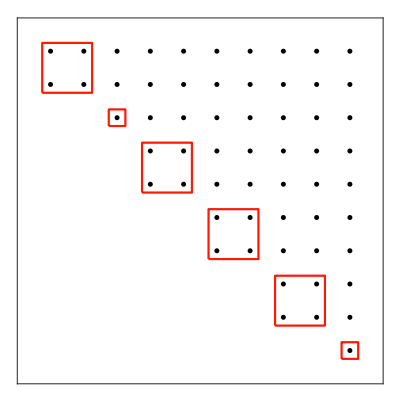
\includegraphics[scale=0.6]{Math_170_Imposter.png}}
            &
            (I did not make this image.\newline Rather it was taken from the\newline class textbook on page 235.) 
         \end{tabular}\retTwo\par}

         We are not going to prove this but the eigenvalues of $\mMat{T}$ are the eigenvalues of each block on the diagonal of $\mMat{T}$.
      \end{myIndent}}
   \end{myIndent}}

   \mySepTwo

   Still, the above algorithm sucks. If the eigenvalues of $\mMat{A}$ are close to each other, it\\ converges really slowly. Plus, taking a QR decomposition every iteration is\\ expensive. So how do we improve this?\retTwo

   Idea:
   {\begin{myIndent} \hTwo
      $\mMat{H} \in \mathbb{R}^{n\times n}$ is called \udefine{upper-Hessenberg} if $h_{i,j} = 0$ for $i > j + 1$.\\ [-13pt]
      {\begin{myIndent} \hFour
         You can think of this as a weaker version of being upper-triangular.\retTwo
      \end{myIndent}}

      \uuline{Theorem}: Every $\mMat{A} \in \mathbb{R}^{n\times n}$ can be decomposed as $\mMat{A} = \mMat{Q}\mMat{H}\mMat{Q}^T$ where $\mMat{Q}$ is\\ orthogonal and $\mMat{H}$ is upper-Hessenberg.\retTwo
      
      {\begin{myIndent} \hThree
         Idea of the algorithm: consider $\mMat{A} = 
         \begin{bmatrix}
            a_{1,1} & \mVecAst{y}^{\phantom{.}T\phantom{.}} \\ \mVecAst{x} & B
         \end{bmatrix}$.\retTwo Create a Householder reflector $\tilde{\mMat{Q}}$ such that $\tilde{\mMat{Q}}\mVec{x} = \|\mVec{x}\|_2e_1$.\retTwo
         Next define $\mMat{Q} = 
         \begin{bmatrix}
            1 & \mVecAst{0}^{\phantom{.}T\phantom{.}} \\ \mVec{0} & \tilde{\mMat{Q}}
         \end{bmatrix}$. Then $\mMat{QAQ}^T = \begin{bmatrix}
            a_{1,1} & \mVecAst{y}^{\phantom{.}T\phantom{.}}\tilde{\mMat{Q}} \\ \tilde{\mMat{Q}}\mVecAst{x} & \tilde{\mMat{Q}}B\tilde{\mMat{Q}}^{\phantom{.}T\phantom{.}}
         \end{bmatrix}$

         \newpage

         Thus, the first column of $\mMat{Q}\mMat{A}\mMat{Q}^T$ has all zero elements after the second row.\retTwo

         Now let $B^\prime = \tilde{\mMat{Q}}B\tilde{\mMat{Q}}^{\phantom{.}T\phantom{.}}$. Inductively, repeat this algorithm on $B^\prime$. Having\\ expressed $B^\prime = \tilde{\mMat{Q}}^\prime H^\prime (\tilde{\mMat{Q}}^\prime)^{\phantom{.}T\phantom{.}}$ where $H^\prime$ is an upper Hessenberg Matrix, define $\mMat{Q}^\prime = \begin{bmatrix}
            \mMat{I}_2 & \mMat{0} \\ \mMat{0} & \tilde{\mMat{Q}}^\prime
         \end{bmatrix}$. Then $\mMat{Q}^\prime\mMat{Q}\mMat{A}\mMat{Q}^T(\mMat{Q}^\prime)^T$ is upper-Hessenberg.\retTwo
      \end{myIndent}}

      Thus we come up with an improved algorithm for QR-iteration.
      \begin{enumerate}
         \item Find an upper-Hessenberg matrix $\mMat{H}$ such that $\mMat{A} = \mMat{QHQ}^T$.
         \item Do QR-iteration on $\mMat{H}$ since $\mMat{H}$ is similar to $\mMat{A}$.\retTwo
         
         {\begin{myTindent} \teachComment
            Note that each $\mMat{H}_k$ obtained by doing QR-iteration on $\mMat{H}$ is also upper-Hessenberg. So the algorithm converges faster. Also,\\ because $\mMat{H}$ has so many zero elements, QR-decomposition only needs $\mathcal{O}(n^2)$ flops. \retTwo

            The total flop count of this algorithm is $\frac{10}{3}n^3 + \mathcal{O}(n^2\cdot N)$ where $n$ is the size of $\mMat{A}$ and $N$ is the number of iterations performed.
         \end{myTindent}}
      \end{enumerate}
   \end{myIndent}}
   \retTwo
   \retTwo
   \retTwo
   \retTwo
   \retTwo
   \retTwo
   \retTwo
   \retTwo
   \retTwo
   \retTwo
   \retTwo
   \retTwo
   \exOne
   Our textbook for the class was \textit{Introduction to Numerical Linear Algebra} by Christoph Börgers.

\end{document}